\documentclass[preprint, 10pt, 5p]{elsarticle}

%% Import packages
\usepackage[nocfg, stdsubgroups]{nomencl}
%\usepackage{setspace}
\usepackage{amsmath, amsfonts}
\usepackage{multirow}
\usepackage{array}
\usepackage{tikz}
\usepackage{pgfplots}
\usepackage{subfig}
\usepackage{threeparttable}
\usepackage{glossaries}

\usepackage[ruled, vlined, linesnumbered]{algorithm2e}
\usepackage{hyperref}

\usepackage[most]{tcolorbox}
\usepackage{multicol} % Multiple columns environment
\renewcommand*\nompreamble{\begin{multicols}{2}}
\renewcommand*\nompostamble{\end{multicols}}


\usepackage{xcolor}
\usepackage{booktabs}
\usepackage{caption}
\usepackage{colortbl}

\definecolor{t1}{RGB}{239, 35, 60} %red
\definecolor{t2}{RGB}{43, 45, 66} %dark grey
\definecolor{t3}{RGB}{141, 153, 174} %light grey

\usetikzlibrary{arrows.meta}
\usetikzlibrary{datavisualization.formats.functions}

%% Defining and loading style of the glossary

\setacronymstyle{long-short}
\loadglsentries{3-acronyms.tex}

\begin{document}
%% Start the first page opening braces with "Frontmatter"

\begin{frontmatter}
%% \title{Title\tnoteref{label1}}
%% \tnotetext[label1]{}

    \title{Implementation of a Microgrid Energy Management System Considering 
    E-Mobility, Uncertainties and Contingencies: A Multi-Objective Approach}

%% \author[label1,label2]{} 

    \author[1]{Derian C. Tairo\corref{corr1}}
    \ead{d255905@dac.unicamp.br}

    \author[1]{Jéssica Alice A. Silva}
    \ead{j262748@dac.unicamp.br}

    \author[2]{Juan Camilo López}
    \ead{j.c.lopezamezquita@utwente.nl}

    \author[1]{Marcos J. Rider}
    \ead{mjrider@unicamp.br}

    \cortext[corr1]{Corresponding author}


%% \affiliation[label1]{organization={},
%%             addressline={},
%%             city={},
%%             postcode={},
%%             state={},
%%             country={}} 
    \affiliation[1]{organization={Department of System and Energy (DSE), School 
        of Electrical and Computer Engineering (FEEC), 
        State University of Campinas (UNICAMP)},
        %addressline={Av. Albert Einstein, 400},
        city={Campinas},
        %postcode={13083-852},
        state={São Paulo},
        country={Brazil}}
    
    \affiliation[2]{organization={Department of Electrical Engineering 
        Mathematics and Computer Science (EEMCS), University of Twente},
        %addressline={Drienerlolaan 5},
        city={Enschede},
        %postcode={7522 NB},
        state={Overijssel},
        country={The Netherlands}}

    \begin{abstract}
        The integration of various \glspl{der}, \glspl{bess}, \gls{pv} systems, 
        and \gls{ev} chargers, introduces new complexities 
        in managing electrical distribution systems. The main challenge 
        involves devising an optimized day-ahead \gls{ems} 
        tailored for three-phase unbalanced AC microgrids while accounting for
        uncertainties in \gls{pv} generation and nodal demands.
        Additionally, the \gls{ems} must prepare the microgrid for potential 
        transitions between grid-connected and islanded modes due to unexpected
        grid outages. The proposed \gls{ems} is specifically designed for 
        microgrids comprising \gls{pv} generation, \gls{bess}, \gls{ev} chargers, and variable demand, facilitating efficient 
        day-ahead planning. Furthermore, the inclusion of contingency 
        constraints ensures a transition between grid-connected and
        islanded modes, augmenting grid resilience. A multi-objective approach is considered to minimize the operation costs from the main grid and energy non-supplied for the EVs.
        To evaluate the proposed EMS, actual data from the \Gls{campus} 
        at the \gls{unicamp} was utilized. 
        The proposed \gls{minlp} model undergoes a
        transformation into a \gls{milp} model through a 
        series of linearizations. The model was implemented using Python 
        Optimization Modeling Objects (Pyomo) and solved using the open-source 
        CBC solver. Results confirm the robustness and efficacy of the proposed 
        \gls{ems} in improving the performance and resilience of three-phase 
        unbalanced AC microgrids.
    \end{abstract}
    \begin{keyword}
        Energy management systems, electric vehicles, microgrid, 
        multi-objective approach.
    \end{keyword}
%% End first page  
\end{frontmatter}

%% Start the next pages

\glsresetall
\section{Introduction}\label{sec:intro}

In a world where sustainability and energy efficiency have become global 
imperatives, effective microgrid management emerges as a revolutionary 
solution to contemporary energy challenges. Microgrids offer crucial 
flexibility in integrating \glspl{res} and enhancing energy 
resilience \cite{uddin2023}. However, the increasing adoption of \glspl{ev} 
and the inherent uncertainty in renewable energy generation poses significant challenges for \gls{ems}. Technologies 
like \gls{iot} provide new opportunities to improve the 
efficiency and adaptability of these systems. 

Microgrids are small electrical networks that can operate isolated or connected
with the main grid, have emerged as a viable solution for 
integrating \glspl{der}, including \glspl{res}, \glspl{bess}, and controllable 
loads \cite{farrokhabadi2020}. In this context, the development and application 
of mathematical models that incorporate real-time analysis 
\cite{yang2019,restrepo2021}, transitions \cite{vergara2019}, 
and three-phase systems \cite{vergara2019_2} 
offer a more accurate and dynamic representation of microgrid behavior.

To address these challenges, it is essential to implement an \gls{ems} that 
can work effectively in microgrids \cite{cimen2022,kim2022}. \gls{ems} are 
designed to monitor, control, and optimize energy use within a microgrid 
\cite{ahmad2023}, 
facilitating the integration not only of \glspl{der} but also of EVs.

%% Print the nomenclature
\begin{figure*}[ht!]
    \begin{tcolorbox}[colframe=black!80!white,colback=white,sharp corners, boxrule=0.5pt, width=\linewidth]%
        \begin{scriptsize}
            %% Make and edits sobgroups the nomenclature
%% To show the nomenclature, in the terminal,  run the following command:
%% makeindex 1-paper.nlo -s nomencl.ist -o 1-paper.nls

\makenomenclature
\renewcommand{\nomgroup}[1]{%
\ifthenelse{\equal{#1}{A}}{\item[\textbf{Sets}]}{%
\ifthenelse{\equal{#1}{B}}{\item[\textbf{Indexes}]}{%
\ifthenelse{\equal{#1}{C}}{\item[\textbf{Parameters}]}{% 
\ifthenelse{\equal{#1}{D}}{\item[\textbf{Continuous Variables}]}{%
\ifthenelse{\equal{#1}{E}}{\item[\textbf{Binary Variables}]}}{}{}{}}}}}

\newcommand{\nomenclspace}[0]{\vspace{-6.5pt}}

\nomenclature[a]{$\mathcal{B}$}{Set of nodes in which a battery energy storage 
    system (BESS) is connected, $\mathcal{B}$ $\subset$ $\mathcal{N}$.\nomenclspace}
\nomenclature[a]{$\mathcal{F}$}{Set of phases {A,B,C}.\nomenclspace}
\nomenclature[a]{$\mathcal{G}$}{Set of nodes in which a thermal generator 
    (genset) unit is connected, $\mathcal{G}$ $\subset$ $\mathcal{N}$.\nomenclspace}
\nomenclature[a]{$\mathcal{L}$}{Set of lines.\nomenclspace}
\nomenclature[a]{$\mathcal{N}$}{Set of nodes.\nomenclspace}
\nomenclature[a]{$\mathcal{C}$}{Set of contingencies.\nomenclspace}
\nomenclature[a]{$\mathcal{T}$}{Set of time intervals.\nomenclspace}
\nomenclature[a]{$\mathcal{S}$}{Set of scenarios.\nomenclspace}
\nomenclature[a]{$\mathcal{V}$}{Set of nodes in which electric vehicles (EVs) 
    chargers are connected, $\mathcal{V}$ $\subset$ $\mathcal{N}$.}

\nomenclature[b]{$c$}{Contingencies $c$ $\in$ $\mathcal{C}$.\nomenclspace}
\nomenclature[b]{$f,h$}{Phases $f$ and $h$ $\in$ $\mathcal{F}$.\nomenclspace}
\nomenclature[b]{$ki,ij$}{Lines $ki$ $\in$ $\mathcal{L}$ and $ij$ $\in$ $\mathcal{L}$.\nomenclspace}
\nomenclature[b]{$i,j$}{Nodes $i$ $\in$ $\mathcal{N}$ and $j$ $\in$ $\mathcal{N}$.\nomenclspace}
\nomenclature[b]{$m$}{Nodes $m$ $\in$ $\mathcal{B}$.\nomenclspace}
\nomenclature[b]{$n$}{Nodes $n$ $\in$ $\mathcal{G}$.\nomenclspace}
\nomenclature[b]{$r$}{Nodes $r$ $\in$ $\mathcal{V}$.\nomenclspace}
\nomenclature[b]{$s$}{Scenarios $s$ $\in$ $\mathcal{S}$.\nomenclspace}
\nomenclature[b]{$t$}{Time intervals $t$ $\in$ $\mathcal{T}$.}

\nomenclature[c]{$\alpha^{\text{C}}$}{Load curtailment cost.\nomenclspace}
\nomenclature[c]{$\alpha_{n}^{\text{G}}$}{Constant operational cost of the 
    genset.\nomenclspace}
\nomenclature[c]{$\alpha_{t}^{\text{S}}$}{Cost of energy imported from the main 
    grid.\nomenclspace}
\nomenclature[c]{$\Delta{t}$}{Duration of each time step.\nomenclspace}
\nomenclature[c]{$\Delta{t}_{c}$}{Duration of each time contingency.\nomenclspace}
\nomenclature[c]{$\eta^{\text{B}}$}{Efficiency of the BESS.\nomenclspace}
\nomenclature[c]{$\overline{{\Delta}^{\text{G}}_{n}}$}{Discretization step for the 
piecewise linearization.\nomenclspace} %of $(P_{n,t,c}^{\text{G}})^2$.\nomenclspace}
\nomenclature[c]{$\overline{{E}^{\text{B}}_{m}}$, $\underline{{E}^{\text{B}}_{m}}$}{Maximum/Minimum energy capacity of the BESS.\nomenclspace}
\nomenclature[c]{$\overline{{P}^{\text{B}}_{m}}$}{Maximum dis/charging limit of the 
BESS.\nomenclspace}
\nomenclature[c]{$\overline{{P}^{\text{G}}_{n}}$, $\underline{{P}^{\text{G}}_{n}}$}{Maximum/Minimum active power of the genset.\nomenclspace}
\nomenclature[c]{$\eta^{\text{EV}}$}{Efficiency of the EV.\nomenclspace}
\nomenclature[c]{$\overline{{E}^{\text{EV}}_{r}}$, $\underline{{E}^{\text{EV}}_{r}}$}{Maximum/Minimum energy capacity of the EV.\nomenclspace}
\nomenclature[c]{$\overline{{P}^{\text{EV}}_{r}}$}{Maximum charging limit of the 
    EV charger.\nomenclspace}
\nomenclature[c]{$\overline{{Q}^{\text{G}}_{r}}$, $\underline{{Q}^{\text{G}}_{n}}$}{Maximum/Minimum reactive power of the genset.\nomenclspace}
\nomenclature[c]{$\sigma_{i,y}$}{Slope of the $y$th block for the piecewise 
    linearization.\nomenclspace}% of $(P_{g,t,c}^{\text{G}})^2$.\nomenclspace}
\nomenclature[c]{$\Tilde{P}_{ij,f,t,c,s}$}{Estimated active power flow.\nomenclspace}
\nomenclature[c]{$\Tilde{Q}_{ij,f,t,c,s}$}{Estimated reactive power flow.\nomenclspace}
\nomenclature[c]{$\Tilde{V}_{i,f,t,c,s}$}{Estimated value of the voltage 
    magnitude.\nomenclspace}

\nomenclature[c]{$\overline{{V}}, \underline{{V}}$}{Maximum/Minimum voltage 
    magnitude.\nomenclspace}
\nomenclature[c]{${E}^{\text{B}_{0}}_{m}$}{Initial energy of the BESS.\nomenclspace}
\nomenclature[c]{${E}^{\text{EV}_{0}}_{r}$}{Initial energy of the EV.\nomenclspace}
\nomenclature[c]{${P}^{\text{D}}_{i,f,t}$}{Profile active power load.\nomenclspace}
\nomenclature[c]{${P}^{\text{D}}_{i}$}{Nominal active power load.\nomenclspace}
\nomenclature[c]{${Q}^{\text{D}}_{i,f,t}$}{Profile reactive power load.\nomenclspace}
\nomenclature[c]{${Q}^{\text{D}}_{i}$}{Nominal reactive power load.\nomenclspace}
\nomenclature[c]{${P}^{\text{PV}}_{i}$}{Nominal active power PV generation.\nomenclspace}
\nomenclature[c]{${P}^{\text{PV}}_{i,f,t}$}{Profile active power PV generation.\nomenclspace}
\nomenclature[c]{${R}^{'}_{ij,f,h}$}{Transformed circuit resistance.\nomenclspace}
\nomenclature[c]{${X}^{'}_{ij,f,h}$}{Transformed circuit reactance.\nomenclspace}
\nomenclature[c]{${Z}^{'}_{ij,f,h}$}{Transformed circuit impedance.}
\nomenclature[c]{${t}_{a}$}{EV time arrival.\nomenclspace}
\nomenclature[c]{${t}_{d}$}{EV time departure.\nomenclspace}
\nomenclature[c]{${Prob}_{s}$}{Probability of scenario.\nomenclspace}
\nomenclature[c]{${V}^{nom}$}{Nominal voltage.\nomenclspace}
\nomenclature[c]{$\overline{{I}^{\text{PCC}}}$}{Maximum current of the PCC.\nomenclspace} % revisar
\nomenclature[c]{$\overline{{S}^{\text{PCC}}_{i}}$}{Maximum power of the PCC.\nomenclspace} 
\nomenclature[c]{${S}^{\text{sub}}$}{Total capacity of transformers.\nomenclspace}
\nomenclature[c]{$Y$}{Number of discrete blocks for the piecewise linearization.\nomenclspace}

\nomenclature[c]{${L}^{B}(m)$}{Node to which the BESS is connected.\nomenclspace}
\nomenclature[c]{${L}^{G}(n)$}{Node to which the genset is connected.\nomenclspace}
\nomenclature[c]{${L}^{V}(r)$}{Node to which the EV charger is connected.\nomenclspace}
\nomenclature[c]{${\gamma^{\text{D}}_{s}}$}{Coefficient for each active and reactive power load scenario.\nomenclspace}
\nomenclature[c]{${\gamma^{\text{PV}}_{s}}$}{Coefficient for each PV generation scenario.\nomenclspace}

\nomenclature[d]{$\Delta^{\text{P}}_{i,t,c,y}$}{Values of the $y$th block used 
    for the piecewise linearization $(P_{ij,f,t,c,s})^2$.\nomenclspace}
\nomenclature[d]{$\Delta^{\text{Q}}_{i,t,c,y}$}{Values of the $y$th block used 
    for the piecewise linearization $(Q_{ij,f,t,c,s})^2$.\nomenclspace}
    \nomenclature[d]{$E^{\text{EV}}_{r,t}$}{Energy of the EV.\nomenclspace}
    \nomenclature[d]{$P^{\text{EV}}_{r,t}$}{Active power injection of the EV.\nomenclspace}
\nomenclature[d]{$P^{\text{EV}+}_{r,f,t}$}{Single-phase charging active power of the EV 
            charger.\nomenclspace}
\nomenclature[d]{$P^{\text{EV}+}_{r,t}$}{Three-phase charging active power of the EV 
    charger.\nomenclspace}
\nomenclature[d]{$E^{\text{B}}_{m,t}$}{Energy of the BESS.\nomenclspace}
\nomenclature[d]{$P^{\text{B}}_{m,t}$}{Active power injection of the BESS.\nomenclspace}    
\nomenclature[d]{$P^{\text{B}+}_{m,f,t}$}{Single-phase charging active power of the 
    BESS.\nomenclspace}
\nomenclature[d]{$P^{\text{B}+}_{m,t}$}{Three-phase charging active power of the BESS.\nomenclspace}
\nomenclature[d]{$P^{\text{B}-}_{m,f,t}$}{Single-phase discharging active power of the 
    BESS.\nomenclspace}
\nomenclature[d]{$P^{\text{B}-}_{m,t}$}{Three-phase discharging active power of the 
    BESS.\nomenclspace}
\nomenclature[d]{$P^{\text{G}}_{n,f,t,c,s}$}{Active power of genset at phase $f$.\nomenclspace}
\nomenclature[d]{$P^{\text{G}}_{n,t,c,s}$}{Total active power of the genset.\nomenclspace}
\nomenclature[d]{$Q^{\text{G}}_{n,f,t,c,s}$}{Reactive power of the genset at 
    phase $f$.\nomenclspace}
\nomenclature[d]{$Q^{\text{G}}_{n,t,c,s}$}{Total reactive power of genset.\nomenclspace}
\nomenclature[d]{$P^{\text{L}}_{ij,f,t,c,s}$}{Active power losses through the 
    circuits.\nomenclspace}
\nomenclature[d]{$Q^{\text{L}}_{ij,f,t,c,s}$}{Reactive power losses through the 
    circuits.\nomenclspace}

\nomenclature[d]{$P^{\text{PCC}}_{i,f,t,c,s}$}{Active power at the PCC.\nomenclspace}
\nomenclature[d]{$Q^{\text{PCC}}_{i,f,t,c,s}$}{Reactive power at the PCC.\nomenclspace}
\nomenclature[d]{$P^{\text{PCCsqr}}_{ij,f,t,c,s}$}{Linear variable used to 
    represent $P^{\text{PCC}}_{i,f,t,c,s}$.\nomenclspace}
\nomenclature[d]{$Q^{\text{PCCsqr}}_{ij,f,t,c,s}$}{Linear variable used to 
    represent $Q^{\text{PCC}}_{i,f,t,c,s}$.\nomenclspace}
\nomenclature[d]{$P^{\text{PCC}+}_{i,f,t,c,s}$}{Positive component for the piecewise 
    linearization of $P^{\text{PCC}}_{i,f,t,c,s}$.\nomenclspace}
\nomenclature[d]{$P^{\text{PCC}-}_{i,f,t,c,s}$}{Negative component for the piecewise 
    linearization of $P^{\text{PCC}}_{i,f,t,c,s}$.\nomenclspace}
\nomenclature[d]{$Q^{\text{PCC}+}_{i,f,t,c,s}$}{Positive component for the piecewise 
    linearization of $Q^{\text{PCC}}_{i,f,t,c,s}$.\nomenclspace}
\nomenclature[d]{$Q^{\text{PCC}-}_{i,f,t,c,s}$}{Negative component for the piecewise 
    linearization of $Q^{\text{PCC}}_{i,f,t,c,s}$.\nomenclspace}

\nomenclature[d]{$P_{ij,f,t,c,s}$}{Active power flow through the circuits.\nomenclspace}
\nomenclature[d]{$Q_{ij,f,t,c,s}$}{Reactive power flow through the circuits.\nomenclspace}
\nomenclature[d]{$P^{\text{sqr}}_{ij,f,t,c,s}$}{Linear variable used to 
    represent $(P_{ij,f,t,c,s})^2$.\nomenclspace}
\nomenclature[d]{$Q^{\text{sqr}}_{ij,f,t,c,s}$}{Linear variable used to 
    represent $(Q_{ij,f,t,c,s})^2$.\nomenclspace}
\nomenclature[d]{$P^{\text{+}}_{ij,f,t,c,s}$}{Positive component for the piecewise 
    linearization of $(P_{ij,f,t,c,s})^2$.\nomenclspace}
\nomenclature[d]{$P^{\text{-}}_{ij,f,t,c,s}$}{Negative component for the piecewise 
    linearization of $(P_{ij,f,t,c,s})^2$.\nomenclspace}
\nomenclature[d]{$Q^{\text{+}}_{ij,f,t,c,s}$}{Positive component for the piecewise 
    linearization of $(Q_{ij,f,t,c,s})^2$.\nomenclspace}
\nomenclature[d]{$Q^{\text{-}}_{ij,f,t,c,s}$}{Negative component for the piecewise 
    linearization of $(Q_{ij,f,t,c,s})^2$.\nomenclspace}

\nomenclature[d]{$V_{i,f,t,c,s}$}{Voltage magnitude of the nodes.}
\nomenclature[d]{$V^{\text{sqr}}_{i,t,c,s}$}{Linear variable used to 
    represent $(V_{i,f,t,c,s})^2$. \nomenclspace}

\nomenclature[d]{$P_{i,f,t,c,s}^{+\text{PCC}}$}{Active power imported at the PCC.\nomenclspace}
\nomenclature[d]{$P_{i,f,t,c,s}^{-\text{PCC}}$}{Active power exported at the PCC.\nomenclspace}


\nomenclature[e]{$b^{+}_{m,t}$}{Variable associated with the charge of the BESS.\nomenclspace}
\nomenclature[e]{$b^{-}_{m,t}$}{Variable associated with the discharge of the BESS.}
\nomenclature[e]{$\mu_{i,t,c,s}$}{Operational state of the genset.\nomenclspace}
\nomenclature[e]{$\chi_{i,t,c,s}$}{Variable associated with load curtailment.\nomenclspace}
\nomenclature[e]{$\psi_{i,t,c,s}$}{Variable associated with PV curtailment.\nomenclspace}


\printnomenclature[0.5in]
        \end{scriptsize}
    \end{tcolorbox}
    \end{figure*}


The growing integration of \glspl{ev} into energy distribution systems 
\cite{banol2023, calero2024} has led to the development of several tools and 
models to manage this integration. However, incorporating \glspl{ev} into 
microgrids is crucial for understanding grid impact, enabling energy managers 
to anticipate and mitigate potential issues such as demand peaks and voltage 
fluctuations \cite{gou2022}. These models can assess 
the efficiency of different \gls{ev} charging and discharging strategies, 
optimizing the use of available energy resources 
\cite{kayode2022, masrur2022}.

%% \multicolumn{number of columns}{position}{text}
%% p{6cm} 'Paragraph box" of width 6cm
%% \arraystretch{1.5} % Increase the row height by 1.5
%% \centering % Center the table and is mandatory
%% \multirow{number of rows}{width}{text}
%% Array package
%% m{1cm} produces a column of width 1cm and centers the text vertically
%% >{decl} can be used to insert a command before each cell in a column
%% \resiblox{0.5\textwidth}{!}{table} % Resize the table to 50% for two columns

\renewcommand{\multirowsetup}{\centering} % Center the text in the first column
\renewcommand{\arraystretch}{1.1}

\begin{table*}
\caption{Comparison of the proposed EMS with previous works.}
\label{tab:comparison}
\begin{center}
    \resizebox{\textwidth}{!}{
    \begin{threeparttable}    
    \begin{tabular}{cccccccccccccc}
        % \hline
        \hline
        \multirow{2}{*}{Ref}
            &\multicolumn{3}{c}{Constraints}
            &\multicolumn{1}{c}{Three-phase}
            &\multicolumn{2}{c}{Uncertainty}
            &\multicolumn{1}{c}{Real}
            &\multicolumn{1}{c}{EV}
                &\multicolumn{1}{c}{\multirow{2}{*}{Multi-objective}}
                &\multicolumn{1}{c}{\multirow{2}{*}{GUI\tnote{1}}}
                &\multicolumn{1}{c}{\multirow{2}{*}{Case study}}
            &\multicolumn{1}{c}{Implemented}
            &\multicolumn{1}{c}{Mathematical}
            
                \\
        \cline{2-4}
        \cline{6-7}
            &\multicolumn{1}{c}{\centering Connected}
            &\multicolumn{1}{c}{Islanded}
            &\multicolumn{1}{c}{Transition}
            &\multicolumn{1}{c}{power flow}
            &\multicolumn{1}{c}{\centering Demand}
            &\multicolumn{1}{c}{PV}
            &\multicolumn{1}{c}{\centering time}
            &\multicolumn{1}{c}{\centering charging}
            &&&&\multicolumn{1}{c}{with}
            &\multicolumn{1}{c}{model\tnote{*}}
            \\
        \hline
        \cite{yang2019}&\checkmark& & & &\checkmark&\checkmark&\checkmark&
            \checkmark& & &Experimental Setup&Matlab&Not mencioned\\
        \cite{restrepo2021}&\checkmark&\checkmark&\checkmark& &\checkmark&
            \checkmark&\checkmark&\checkmark& &\checkmark&Real Microgrid&
            Pyomo&MILP\\
        \cite{vergara2019}&\checkmark&\checkmark& &\checkmark&\checkmark&
            \checkmark& & & & &Simulation&AMPL&MISOCP\\
        \cite{vergara2019_2}&\checkmark&\checkmark& &\checkmark&\checkmark&
            \checkmark& & & & &Simulation&AMPL&MINLP\\
        \cite{cimen2022}&\checkmark& & & &\checkmark&\checkmark&\checkmark&
            \checkmark&\checkmark& &Experimental Setup&Matlab&DL\\
        \cite{kim2022}&\checkmark& & & &\checkmark&\checkmark& &\checkmark& 
            &\checkmark&Experimental Setup&Not informed&MINLP\\
        \cite{gou2022}&\checkmark& & & &\checkmark&\checkmark& &\checkmark& & &
            Simulation&Matlab&MIQP\\
        \cite{masrur2022}&\checkmark&\checkmark& & &\checkmark&\checkmark& &
            \checkmark& & &Experimental Setup&Pyomo&MILP\\
        \cite{li2024}&\checkmark& & & &\checkmark&\checkmark& &\checkmark&
            \checkmark& &Simulation&Matlab&ADMM\\
        \cite{zhang2022}&\checkmark& & & & & & &\checkmark&\checkmark& &
            Simulation&Not informed&Heuristic\\
        \cite{mei2022}&\checkmark& & & &\checkmark& & &\checkmark&\checkmark& &
            Simulation&Not informed&Heuristic\\
        \cite{ullah2023}&\checkmark& & & &\checkmark&\checkmark&\checkmark&
            \checkmark& &\checkmark&Experimental&Homer Grid&Heuristic\\
        \cite{pitchai2024}&\checkmark& & & &\checkmark&\checkmark& & & & &
            Simulation&Matlab&Heuristic\\
        \cite{mansouri2023}&\checkmark& & & &\checkmark&\checkmark& &
            \checkmark& & &Simulation&Matlab \& GAMS&MILP\\

        \cite{yehia2024}&\checkmark&\checkmark& & &\checkmark&\checkmark&
            \checkmark& & &\checkmark&Experimental Setup&Matlab/Simulink&
            Not mencioned\\
        \cite{abid24}&\checkmark& & & &\checkmark&\checkmark& &\checkmark&
            \checkmark& &Simulation&Not informed&Metaheuristic\\
        \cite{silva2023}&\checkmark&\checkmark&\checkmark&\checkmark&\checkmark&
            \checkmark&\checkmark& & &\checkmark& Real Microgrid&Pulp&MILP\\
        \cite{zandrazavi2022}&\checkmark& & &\checkmark&\checkmark&\checkmark&
            &\checkmark&\checkmark& &Simulation&AMPL&NLP\\
        This work&\checkmark&\checkmark&\checkmark&\checkmark&\checkmark&
            \checkmark&\checkmark&\checkmark&\checkmark&\checkmark
            &Real Microgrid&Pyomo/Python&MILP\\
                       
        % \hline
        \hline
 
    \end{tabular}
    \begin{tablenotes}
        \item[1] \footnotesize Graphical User Interface.
        \item[*] \footnotesize MINLP - Mixed-Integer Nonlinear Programming,
        MISOCP - Mixed-Integer Second-Order Cone Programming,
        MILP - Mixed-Integer Linear Programming,
        DL - Deep Learning,
        MIQP - Mixed-Integer Quadratic Programming,
        ADMM - Alternating Direction Method of Multipliers,
        RL - Reinforcement Learning,
        NLP - Nonlinear Programming.
    \end{tablenotes}
    \end{threeparttable}
    }
\end{center}
\end{table*}

% Addressing the challenge of minimizing microgrid operation costs while 
% maximizing energy availability for \gls{ev} charging requires a multi-objective 
% approach \cite{wu2023}.
A multi-objective optimization approach allows for balancing different 
priorities, such as, cost reduction, voltage deviation, and 
efficient \gls{ev} charging management \cite{zandrazavi2022, li2024}. 
The use of multi-objective 
optimization algorithms \cite{abid24} in microgrid management 
enable the development of strategies capable of responding to changing demands and 
operational 
uncertainties \cite{zhang2022, mei2022}. Despite incorporating 
multi-objective models, practical implementation in real 
microgrid environments remains limited, highlighting the need 
for new tools.

Frameworks like \gls{iot} facilitate data collection from various devices, 
supporting data analysis and decision-making in \gls{ems} \cite{ullah2023,yehia2024}. 
\gls{iot} integration in \gls{ems} enables continuous and detailed monitoring of 
the microgrid, from energy generation and storage to final 
consumption \cite{pitchai2024}. Connected devices can provide real-time data 
on network operation, environmental conditions, and equipment 
status \cite{mansouri2023}. This information is vital for predictive 
analysis and operational optimization, allowing energy managers to respond 
quickly to changes and ensure continuous network operation.

In continuation of the work by \cite{silva2023}, which considers transitions 
from an isolated to a connected system or vice versa, a three-phase AC system, 
real-time operation, and an IoT-based EMS, this work presents several 
advancements. Unlike the previous work, which did not consider the development 
of \glspl{ev} or a multi-objective approach, this work introduces a 
multi-objective stochastic approach. It aims to minimize network costs and 
\gls{ens} for \glspl{ev}, considering uncertainties in \gls{pv} generation 
and demand. We developed six case studies to evaluate the performance of the 
EMS, all validated with real data from the \gls{campus} at the \gls{unicamp}.
The main contributions of this work 
are:

\begin{itemize}
    \item A \gls{moop} approach that minimizes operational costs from the main 
    grid and \gls{ens} for \glspl{ev}. The \gls{moop} is addressed using the 
    $\epsilon$-constraint method.

    \item The adaptability of a new window in the IoT-based EMS, this feature 
    allows \gls{ev} owners to input their arrival and departure times, 
    enabling the EMS to plan EV charging according to their needs.

    \item Validation through real-time simulation using HIL, considering 
    contingencies and the operation of \glspl{ev}.

\end{itemize} 

For a better understanding of the problem, Table 
\ref{tab:comparison} summarizes the literature review.

The structure of this paper is organized as follows: Section \ref{sec:intro} 
introduces the challenges and objectives of the study. 
Section \ref{sec:methodology} describes the methodology, detailing the 
multi-objective mathematical model. 
Section \ref{sec:architecture}, the \gls{ems} software architecture is analyzed, 
including the new window for the \glspl{ev}. Sections \ref{sec:case_study} and \ref{sec:tests_results} 
present the case studies and results. 
Finally, section \ref{sec:conclusions} concludes the paper, 
highlighting the main contributions and suggesting future research and 
development directions.

\section{Methodology}\label{sec:methodology}

Given the unpredictable nature of solar generation, variable demand,
and the increasing integration of \glspl{ev} into microgrids, 
we face challenges that require adaptable and innovative solutions. 
To address these challenges, we have developed an efficient \gls{ems}. 
This system combines stochastic analysis of 
uncertainties for solar generation and demand, three-phase mathematical 
modeling with constraints to ensure optimal microgrid performance under 
various conditions, and multi-objective optimization. 

%% \subfloat[listentry][subcaption]{body}
%% \begin{axis}[<options>]<enviroment contents>\end{axis}
%% \add plot [<options>] table [<column selection>]{<file or inline table>}

\begin{figure*}[htb!]
    \centering
    \subfloat[Scenarios for solar generation and demand]{%
        \begin{tikzpicture}[baseline]
    \begin{axis}[
    xlabel={Period time [h]},
    ylabel near ticks,
    xlabel near ticks,
    ylabel={Active Power [p.u.]},
    tick style = {line width = 0.5, color = lightgray, 
        major tick length=4pt,minor tick length=2pt,
        minor x tick num = 3, minor y tick num =1},
    tick label style = {font=\small, xtick distance=4, ytick distance=152,
        xticklabels={00:00, 00:00, 04:00, 08:00, 12:00, 16:00, 20:00},
        yticklabels={0,0,0.2,0.4,0.6,0.8,1.0}},
    legend style = {font=\footnotesize, at={(0.99,0.98)}, 
        legend cell align=left, line width=0.5pt, draw=lightgray},
    legend entries={High PV, Medium PV, Low PV, High load, Medium load, Low load},
    ymin=0, ymax=760,
    xmin=0, xmax=23,
    width=11.5cm,
    height=7.5cm,
    axis line style = {lightgray, line width = 0.5pt},
    cycle multi list={
    black, gray\nextlist
    linestyles
    }
    ]

    \addplot  table 
        [col sep=comma, x=h, y=pv_h] {./Data/pv_pd.dat};
    % \addlegendentry{High PV}

    \addplot  table 
        [col sep=comma, x=h, y=pv_m] {./Data/pv_pd.dat};
    % \addlegendentry{Medium PV}

    \addplot  table 
        [col sep=comma, x=h, y=pv_l] {./Data/pv_pd.dat};
    % \addlegendentry{Low PV}

    \addplot  table 
        [col sep=comma, x=h, y=pd_h] {./Data/pv_pd.dat};
    % \addlegendentry{High load}

    \addplot  table 
        [col sep=comma, x=h, y=pd_m] {./Data/pv_pd.dat};
    % \addlegendentry{Medium load}

    \addplot  table 
        [col sep=comma, x=h, y=pd_l] {./Data/pv_pd.dat};
    % \addlegendentry{Low load} 
    \end{axis}
\end{tikzpicture}
        \label{fig:scenarios}
    }
    \hfill
    \subfloat[Set of contingencies]{
        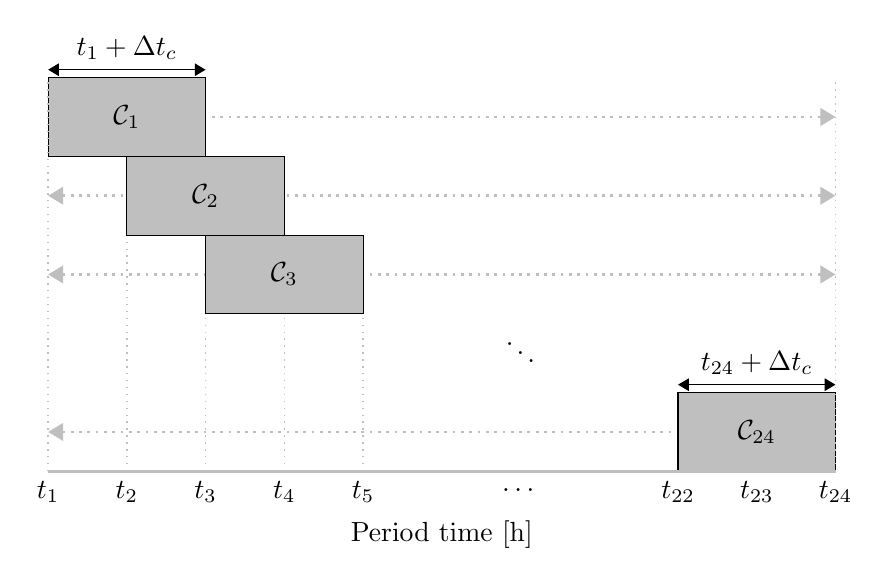
\begin{tikzpicture}[xscale=2, yscale=1, baseline]
    % \draw[help lines] (0,0) grid (5,5);

    %grid lines
    \draw [lightgray, dotted, line width=1, <->][Triangle-Triangle] 
            (0,4.5) -- (5,4.5);
    \draw [lightgray, dotted, line width=1, <->][Triangle-Triangle] 
            (0,3.5) -- (5,3.5);
    \draw [lightgray, dotted, line width=1, <->][Triangle-Triangle] 
            (0,2.5) -- (5,2.5);
    \draw [lightgray, dotted, line width=1, <->][Triangle-Triangle] 
            (0,0.5) -- (5,0.5);

    \draw [lightgray, dotted, line width=0.5] 
            (0.5,0) -- (0.5,3);
    \draw [lightgray, dotted, line width=0.5] 
            (1,0) -- (1,2);
    \draw [lightgray, dotted, line width=0.5] 
            (1.5,0) -- (1.5,2);
    \draw [lightgray, dotted, line width=0.5] 
            (2,0) -- (2,2);

    \node[below] at (3,2) {$\ddots$};

    % body
    \draw [fill=lightgray] (0,4) rectangle (1,5);
        \draw [black, line width=0.5, <->][Triangle-Triangle] 
            (0,5.1) -- (1,5.1);
        \node [above] at (0.5,5.1) {$t_{1} + \Delta t_{c}$};
            \node at (0.5,4.5) {$\mathcal{C}_{1}$};

    \draw [fill=lightgray] (0.5,3) rectangle (1.5,4);
        %\draw [black, line width=0.5, <->][Triangle-Triangle] 
        %   (1,4.1) -- (2,4.1);
        %\node [above] at (1.5,4) {$t_{2} + \Delta t_{c}$};
            \node at (1,3.5) {$\mathcal{C}_{2}$};

    \draw [fill=lightgray] (1,2) rectangle (2,3);
        %\draw [black, line width=0.5, <->][Triangle-Triangle]
        %    (2,3.1) -- (3,3.1);
        %\node [above] at (2.5,3) {$t_{3} + \Delta t_{c}$};
            \node at (1.5,2.5) {$\mathcal{C}_{3}$};
    % \draw [dotted, line width=1] (3,2) -- (4,1);

    \draw [fill=lightgray] (4,0) rectangle (5,1);
        \draw [black, line width=0.5, <->] [Triangle-Triangle] 
            (4,1.1) -- (5,1.1);
        \node [above] at (4.5,1.1) {$t_{24} + \Delta t_{c}$};
            \node at (4.5,0.5) {$\mathcal{C}_{24}$};

    %axis lines        
    \draw [lightgray, dotted, line width=0.5]  (0,0) -- (0,5);
    \draw [lightgray, dotted, line width=0.5]  (5,0) -- (5,5);
    \draw [lightgray, line width=1 ] (0,0) -- (5,0);
    %\draw [black, line width=1 ] (0,5.5) -- (5,5.5);

    % x labels
    \node[below] at (0,0) {$t_1$};
    \node[below] at (0.5,0) {$t_2$};
    \node[below] at (1,0) {$t_3$};
    \node[below] at (1.5,0) {$t_4$};
    \node[below] at (2,0) {$t_5$};
    \node[below] at (4,0) {$t_{22}$};
    \node[below] at (4.5,0) {$t_{23}$};
    \node[below] at (5,0) {$t_{24}$};
    \node[below] at (3,-0.1) {$\dotsc$};

    \node[below] at (2.5,-0.5) {$\text{Period time [h]}$};    
\end{tikzpicture}
        \label{fig:outages}
        }
    \caption{Generation of the set of scenarios (\ref{fig:scenarios}) and 
        contingencies (\ref{fig:outages}).}
    \label{fig:scenarios and outages}
\end{figure*}

\subsection{Uncertainty and Contingency Sets}

To deal with the uncertainties of the problem, we utilize various profiles 
for solar generation and demand. We apply three profiles: 
high, medium, and low, for both solar generation and demand over a 24-hours 
period. This results in a total of nine combined scenarios that 
form the base of the stochastic analysis. Fig. \ref{fig:scenarios} illustrates
these scenarios.

Furthermore, failures in the main power grid can occur anytime, forcing the 
microgrid to operate islanded. In this sense,  set $\mathcal{C}$ includes 
all the possibilities of occurrence of a contingency. 
The model considers a set of 
24 contingencies that reflect all time intervals \{1, ... , 24\}, 
each potentially occurring at any hour within the 24-hour interval. 
Each contingency lasts for two hours ($\Delta t_c$), after which the microgrid 
reconnects to the main grid, see Fig. \ref{fig:outages}.

\subsection{Mathematical Model for the EMS}

% The EMS problem can be modeled as a MINLP model given by 
% \eqref{obj_1}-\eqref{EV_out}. 
The \gls{ems} mathematical model is formulated as a \gls{minlp} 
model, encompassing two objectives functions and constraints related to the 
three-phase operation of the microgrid under various scenarios and 
contingencies. The main purpose of the \gls{ems} is to find the best solution, minimizing 
operational costs from the main grid and the \gls{ens} for \glspl{ev}. 
In sequence, a set of linearizations is used to transform the 
\gls{minlp} into a \gls{milp} model, this transformation is detailed in
\ref{appndx:piecewise}.

Into to \gls{milp} model, the continuous decision variables are the active and reactive power 
imported/exported at the \gls{pcc} ($P_{i,f,t,c,s}^{PCC}$, 
$Q_{i,f,t,c,s}^{PCC}$), the active and reactive 
power of the genset ($P_{n,t,c,s}^{G}$, $Q_{n,t,c,s}^{G}$), the active power 
injection of the \gls{bess} ($P_{m}^{B}$) and the active power injection of 
the \gls{ev} ($P_{r}^{EV}$).

Moreover, the binary decision variables represent load curtailment and \gls{pv}
disconnection ($\chi_{i,t,c,s}$), as well as the operational state of 
the genset ($\mu_{i,t,c,s}$). To simplify and reduce the solution time of 
the optimization problem, a single binary variable is used to denote both 
load curtailment and \gls{pv} disconnection. However, it is important to 
note that this variable does not simultaneously perform load curtailment 
and \gls{pv} disconnection, as these actions occur at different nodes within 
the system.

\subsubsection{Objective function 1}

The first objective function, given by \eqref{obj_1}, seeks to minimize the 
operational costs of the microgrid for a day-ahead scheduling. 
The first term refers to the cost of purchasing electricity 
from the main grid. The second term calculates the costs of the \gls{genset} 
operation, and the third term penalizes any load curtailment. 


\vspace{-15pt}
\begin{multline}\label{obj_1}
{f_{costs}} = \min \Delta t \sum_{s \in \mathcal{S}} 
    \Biggl\{ \mathit{Prob}_{s} \cdot \Bigg[
        \sum_{i \in \mathcal{N}} 
        \sum_{f \in \mathcal{F}} 
        \sum_{t \in \mathcal{T}} 
        \sum_{c \in \mathcal{C}} 
\alpha_{t}^{\text{S}} P_{i,f,t,c,s}^{\text{PCC}}  \\
    + \sum_{n \in \mathcal{G}} 
    \sum_{t \in \mathcal{T}} 
    \sum_{c \in \mathcal{C}} 
\Big(P^{\text{G}}_{n,t,c,s} \cdot \alpha_{n}^{\text{G}} \cdot \mu_{n,t,c,s} \Big)  \\
    + \sum_{i \in \mathit{N}} 
    \sum_{f \in \mathit{F}}
    \sum_{t \in \mathit{T}}
    \sum_{c \in \mathit{C}} \alpha^{\text{C}} P_{i,f,t}^{\text{D}} 
        (1 - x_{i,f,t,c}) \Bigg] \Biggr\} 
\end{multline}
\vspace{-12pt}

\subsubsection{Objective function 2}

The second objective function, given by \eqref{obj_2}, aims to minimize the 
\gls{ens} to each \gls{ev} during the hours that coincides with their 
departure times.  This ensures that the \glspl{ev} receive sufficient charging, 
even for intervals of one or two hours, thereby guaranteeing their 
availability when needed by the \gls{ev} owner.

\begin{equation}\label{obj_2}
{f_{ens}} = \min \sum_{\forall r,t | t=t_{d}} 
    \left( \overline{{E}_{r}^{\mathrm{EV}}} - {E}_{r,t}^{\mathrm{EV}} \right)
\end{equation}

\subsubsection{Constraints related to the operation of three-phase distribution systems}

The three-phase unbalanced AC power flow is given by 
(\ref{P_flow})–(\ref{pcc}). 
Constraints (\ref{P_flow}) and (\ref{Q_flow}) 
represent the active and reactive power balance in the microgrid. 
Constraints (\ref{P_losses}) and (\ref{Q_losses}) 
calculate the active and reactive power losses at each circuit. 
Eq. (\ref{V_drop}) calculates the voltage 
magnitude through the circuits.
Voltage limits are guaranteed by (\ref{V_limit}), while (\ref{V_nom}) 
fixes the voltage magnitude of the PCC node.  
Current limits are given by (\ref{I}) and (\ref{pcc}) represents 
the substation capacity.

\vspace{-10pt}
\begin{multline}\label{P_flow}
    \hspace{-10pt}\sum_{ki\in {L}} P_{ki,f,t} 
    - \sum_{ij\in \mathcal{L}} \Big(P_{ij,f,t} + P^{\text{L}}_{ij,f,t} \Big) + 
    P^\text{S}_{i,f,t} + \\ 
    \hspace{-110pt}\sum_{n\in \mathcal{G} |i=L^G(n)}\!\!\!\!\!\!\! 
    P^{\text{G}}_{n,f,t}
    = P^\text{D}_{i,f,t} - P^\text{PV}_{i,f,t} +\\ \!\!\!\!\!\!\!
    \sum_{m\in \mathcal{B} |i=L^B(m)}\!\!\!\!\!\!\! P^{\text{B}}_{m,t} + 
    \!\!\!\!\!\sum_{r\in \mathcal{V} |i=L^{\text{EV}}(r)}\!\!\!\!\!\!\! 
    P^{\text{\text{EV}}}_{r,f,t}
    \quad  \forall i,f,t
\end{multline}
\vspace{-25pt}

\begin{multline}\label{Q_flow}
    \hspace{-10pt}\sum_{ki\in \mathcal{L}} Q_{ki,f,t} - 
    \sum_{ij\in \mathcal{L}} \Big(Q_{ij,f,t} + Q^{\text{L}}_{ij,f,t} \Big) + 
    Q^\text{S}_{i,f,t} + \\
    \sum_{n\in \mathcal{G} |i=L^G(n)}\!\!\!\!\!\!\! Q^{\text{G}}_{n,f,t} = 
    Q^\text{D}_{i,f,t}  \quad \forall i,f,t
\end{multline}
\vspace{-35pt}
  
\begin{multline}\label{P_losses}
    P^{\text{L}}_{ij,f,t} = \\
        \sum_{h \in \mathcal{F}} 
        \frac{1}{V_{i,f,t}V_{i,h,t}}\bigg[ R'_{ij,f,h}\Big(P_{ij,h,t}P_{ij,f,t}  
    + Q_{ij,h,t}Q_{ij,f,t}\Big)\\ + X'_{ij,f,h} \Big( Q_{ij,h,t}P_{ij,f,t} 
    - P_{ij,h,t}Q_{ij,f,t}\Big) \bigg] \quad \forall ij,f,h,t
\end{multline}
\vspace{-35pt}
        
\begin{multline}\label{Q_losses}
    Q^{\text{L}}_{ij,f,t} = \\
        \sum_{h \in \mathcal{F}} 
        \frac{1}{V_{i,f,t}V_{i,h,t}}\bigg[ R'_{ij,f,h}\Big(P_{ij,h,t}Q_{ij,f,t} 
    - Q_{ij,h,t}P_{ij,f,t}\Big) \\ 
    + X'_{ij,f,h} \Big( P_{ij,h,t}P_{ij,f,t} 
    + Q_{ij,h,t}Q_{ij,f,t}\Big)  \bigg] \quad \forall ij,f,h,t
\end{multline}
\vspace{-35pt}

\begin{multline}\label{V_drop}
\hspace{-10pt}V^{\text{2}}_{i,f,t} - V^{\text{2}}_{j,f,t}  =
    2 \sum_{h \in \mathcal{F}} \left(  R'_{ij,f,h} P_{ij,h,t} +
    X'_{ij,f,h} Q_{ij,h,t} \right) -\\
\hspace{-40pt}\frac{1}{V^{\text{2}}_{i,f,t}} 
    \left[\sum_{h \in \mathcal{F}}\left(R'_{ij,f,h}P_{ij,h,t} + 
    X'_{ij,f,h}Q_{ij,h,t}\right) \right]^2-\\ 
\hspace{-10pt}\frac{1}{V^{\text{2}}_{i,f,t}}
    \left[\sum_{h \in \mathcal{F}}\left(R'_{ij,f,h}Q_{ij,h,t} - 
    X'_{ij,f,h}P_{ij,h,t}\right) \right]^2 \forall ij,f,h,t
\end{multline}
\vspace{-30pt}

\begin{flalign}\label{V_limit}
    &\underline{{V}_{t}}  \leq  V_{i,f,t}\leq  \overline{{V}_{t}}& \quad 
    \forall i,f,t &
\end{flalign}
\vspace{-40pt}

\begin{flalign}\label{V_nom}
    &V_{i,f,t} = {V}_{t}^{\text{nom}}&  \quad \forall i,f,t &
\end{flalign}
\vspace{-35pt}
    
\begin{flalign}\label{I}
    &\frac{\left(P^{2}_{ij,f,t} + Q^{2}_{ij,f,t}\right)}{V^{2}_{i,f,t}}  
    \leq \overline{I}_{ij}^2& \quad \forall ij,f,t &
\end{flalign}
\vspace{-30pt}
    
\begin{flalign}\label{pcc}
    &\left( P_{i,f,t,c}^{\text{PCC}} \right)^2 + (Q_{i,f,t,c}^{\text{PCC}})^2 
    \leq (\overline{{S}^{\text{PCC}}})^2& \quad \forall i,f,t,c &
\end{flalign}

\subsubsection{Constraints related to genset operation}

Eqs. (\ref{P_G})–(\ref{QG_limits}) model the operation of the \gls{genset}. 
Constraints (\ref{P_G}) and (\ref{Q_G}) define the total active and reactive 
power output of each phase, and (\ref{PG_limits}) and (\ref{QG_limits}) impose 
the active and reactive power limits.
\vspace{-6pt}
\begin{flalign}\label{P_G}
& P^{\text{G}}_{n,t} =  \sum_{f \in \mathcal{F}} P^{\text{G}}_{n,f,t}&
 \qquad \forall n,f,t 
\end{flalign}
\vspace{-30pt}

\begin{flalign}\label{Q_G}
& Q^{\text{G}}_{n,t} =  \sum_{f \in \mathcal{F}} Q^{\text{G}}_{n,f,t}&
 \qquad \forall n,f,t &
\end{flalign}
\vspace{-30pt}

\begin{flalign}\label{PG_limits}
& \underline{{P}^{\text{G}}_n} \cdot u_{n,t} \leq P^{\text{G}}_{n,t} 
\leq \overline{{P}^{\text{G}}_n}  \cdot u_{n,t}& \qquad 
  \forall n,f,t &
\end{flalign}
\vspace{-35pt}

\begin{flalign}\label{QG_limits}
& \underline{{Q}^{\text{G}}_n} \cdot u_{n,t} \leq Q^{\text{G}}_{n,t} 
\leq \overline{{Q}^{\text{G}}_n}  \cdot u_{n,t}& \qquad  \forall n,f,t &
\end{flalign}

\subsubsection{Constraints related to islanded operation}

The proposed formulation considers unexpected outages of the main grid via 
contingency constraints. In this context, the $\mathcal{C}$is used to indicate a 
contingency. Therefore, the security-constrains (\ref{pcc_1}) and (\ref{pcc_2}) 
model the disconnection of the microgrid to the main grid when $t \geq c$ 
and $t \leq c + \Delta t_{\circ}$.
\vspace{-3pt}
\begin{flalign}\label{pcc_1}
& P_{i,f,t,c}^{\text{PCC}} = 0& \qquad \forall i,f,t,c  | _{ t \geq c \ 
\wedge \ t \leq c + \Delta t_{\circ}} &
\end{flalign}
\vspace{-40pt}

\begin{flalign}\label{pcc_2}
& Q_{i,f,t,c}^{\text{PCC}} = 0& \qquad \forall i,f,t,c  | _{ t \geq c \ 
\wedge \ t \leq c + \Delta t_{\circ}} &
\end{flalign}

\subsubsection{Constraints related to BESS}


Constraints (\ref{B_energy_1})–(\ref{B_lim_EB}) model the operation of the \gls{bess}. 
Note that the \gls{bess} do not depend on the set of contingencies $\mathcal{C}$ because the problem finds the optimal operation of the \gls{bess} in different operating scenarios.
Thus, constraints (\ref{B_energy_1}) and (\ref{B_energy_2}) defines the \gls{soc} of the \gls{bess}, where (\ref{B_energy_1}) depends on the initial energy of 
the \gls{bess} and (\ref{B_energy_2}) depends on the energy stored in the previous 
period ($ E_{m,t-1}^\text{B} $). Constraint (\ref{B_power}) defines the total 
input/output power of the \gls{bess} considering the respective efficiencies. 
Constraint (\ref{B_unimodality}) guarantees that the \gls{bess} do not charge and 
discharge at the same time. Constraints (\ref{B_total_PBd}) and (\ref{B_total_PBc}) 
define the three-phase dis/charging power, whereas (\ref{B_balance_1}) 
and (\ref{B_balance_2}) guarantee a balanced operation. 
Finally, constraints (\ref{B_lim_pch})–(\ref{B_lim_EB}) specify the limits for 
the three-phase dis/charging active power, and the energy according to the 
minimum and maximum capacities, respectively.

\vspace{-12pt}
\begin{flalign}\label{B_energy_1}
& E_{m,t}^\text{B}  = E_{m}^\text{B,\text{ini}}+ P^\text{B}_{m,t} \cdot \Delta t& 
\qquad \forall m,t | _{t = 1} &
\end{flalign}
\vspace{-38pt}

\begin{flalign}\label{B_energy_2}
& E_{m,t}^\text{B}  = E_{m,t-1}^\text{B}+ P^\text{B}_{m,t} \cdot \Delta t& 
\qquad \forall m, t | _{t>1} &
\end{flalign}
\vspace{-38pt}

\begin{flalign}\label{B_power}
& P_{m,t}^\text{B}  = P^\text{B+}_{m,t} \cdot \eta_{m}^\text{B} -
P_{m,t}^\text{B-} \cdot \frac{1}{\eta_{m}^\text{B}}& \qquad \forall m, t & 
\end{flalign}
\vspace{-38pt}

\begin{flalign}\label{B_unimodality}
& P^\text{B+}_{m,t} \cdot P_{m,t}^\text{B-} = 0& \qquad \forall m, t & 
\end{flalign}
\vspace{-38pt}

\begin{flalign}\label{B_total_PBd}
& P^{\text{B-}}_{m,t} =  \sum_{f \in \mathcal{F}} P^{\text{B-}}_{m,f,t}&
\qquad \forall m,t &
\end{flalign}
\vspace{-32pt}

\begin{flalign}\label{B_total_PBc}
& P^{\text{B+}}_{m,t} =  \sum_{f \in \mathcal{F}} P^{\text{B+}}_{m,f,t}&
\qquad  \forall m, t &
\end{flalign}
\vspace{-32pt}

\begin{flalign}\label{B_balance_1}
& P^{\text{B+}}_{m,f,t} =  P^{\text{B+}}_{m,h,t}& \qquad \forall m, f, h, t &
\end{flalign}
\vspace{-38pt}

\begin{flalign}\label{B_balance_2}
& P^{\text{B-}}_{m,f,t} =  P^{\text{B-}}_{m,h,t}& \qquad  \forall m, f, h, t&
\end{flalign}
\vspace{-38pt}

\begin{flalign}\label{B_lim_pch}
& 0 \leq P^{\text{B+}}_{m,t} \leq \overline{{P}^{\text{B}}_{m}}&
\qquad  \forall m, t &
\end{flalign} 
\vspace{-38pt}

\begin{flalign}\label{B_lim_pdis}
& 0 \leq P^{\text{B-}}_{m,t} \leq \overline{{P}^{\text{B}}_{m}} &
\qquad   \forall m, t &
\end{flalign}
\vspace{-38pt}

\begin{flalign}\label{B_lim_EB}
& \underline{{E}^{\text{B}}_{m}} \leq E^{\text{B}}_{m,t} \leq 
\overline{{E}^{\text{B}}_{m}}& \qquad  \forall m, t &
\end{flalign}

\subsubsection{Constraints related to EVs}

Constraints (\ref{EV_1})–(\ref{EV_out}) model the operation of the \gls{ev} chargers. 
Once again, the operation of the \glspl{ev} does not depend on the set of outages. 
Thus, constraints (\ref{EV_1}) and (\ref{EV_2}) define the state of charge of the \glspl{ev}. The three-phase charging power is defined by (\ref{EV_total_PBc}) and 
the balanced injection is enforced by (\ref{EV_balance_1}). 
Constraints (\ref{EV_lim_pch}) and (\ref{EV_lim_EB}) specify the limits for the three-phase charging power, and the energy according to the minimum and maximum 
\gls{ev} capacities. Eq. (\ref{EV_out}) imposes that no \gls{ev} charge is deployed outside $t_{a}$ and $t_{d}$.

\vspace{-15pt}
\begin{flalign}\label{EV_1}
& E_{r,t}^\text{EV}  = E_{r}^\text{EV,\text{ini}}+ 
P^\text{EV}_{r,t} \cdot \eta_{r}^\text{EV} \cdot \Delta t&   \qquad 
\forall r,t | _{t = t_{a}} &
\end{flalign}
\vspace{-35pt}

\begin{flalign}\label{EV_2}
 & E_{r,t}^\text{EV}  = E_{r,t-1}^\text{EV} + 
 P^\text{EV}_{r,t} \cdot \eta_{r}^\text{EV} \cdot \Delta t&  \ \ \quad 
 \forall r, t  | _{ t > t_{a} \ \wedge \ t \leq t_d} &
\end{flalign}
\vspace{-35pt}

\begin{flalign}\label{EV_total_PBc}
& P^{\text{EV+}}_{r,t} =  \sum_{f \in \mathcal{F}} P^{\text{EV+}}_{r,f,t}&
 \qquad \forall r,t | _{ t > t_{a} \ \wedge \ t \leq t_d} &
\end{flalign}
\vspace{-30pt}

\begin{flalign}\label{EV_balance_1}
& P^{\text{EV+}}_{r,f,t} =  P^{\text{EV+}}_{r,h,t}& \qquad  
\forall r,f,h,t | _{t > t_{a} \ \wedge \ t \leq t_d} &
\end{flalign}
\vspace{-35pt}

\begin{flalign}\label{EV_lim_pch}
& 0 \leq P^{\text{EV+}}_{r,t} \leq \overline{{P}^{\text{EV}}_{r}}&   \qquad \ 
\forall r, t | _{ t > t_{a} \ \wedge \ t \leq t_d} &
\end{flalign}
\vspace{-35pt}

\begin{flalign}\label{EV_lim_EB}
& \underline{{E}^{\text{EV}}_{r}} \leq E^{\text{EV}}_{r,t} \leq 
\overline{{E}^{\text{EV}}_{r}} &  \qquad 
\forall r, t | _{ t > t_{a} \ \wedge \ t \leq t_d} &
\end{flalign}
\vspace{-35pt}

\begin{flalign}\label{EV_out}
& P^{\text{EV+}}_{r,f,t} = 0&  
\forall r,f,t | _{ t < t_{a} \ \wedge \ t \geq t_d} & 
\end{flalign}

\subsection{Multi-objective Optimization Problem}\label{subsec:moop}

A \gls{moop} involves more than one objective function to be minimized or maximized, where the answer is a set of solutions defining the best trade-off between the objectives. In this context, dominance determines the solution for the \gls{moop}. For instance, solution $x_1$  dominates $x_2$ if $x_1$ is no worse 
than $x_2$ in both objectives and strictly better than $x_2$ in at least one objective. If either of these conditions is violated, we have non-dominated solutions \cite{deb11}.

Given a set of solutions, the non-dominated solutions are those not dominated 
by any other solution. This set is called the Pareto-optimal set. 
The boundary formed by these points is known as the Pareto-optimal front or 
optimal trade-off surface \cite{boyd2004}.

To solve the \gls{moop}, we employ the $\varepsilon$-constraint method. 
This technique is widely recognized for its simplicity and applicability 
in \gls{moop} \cite{chiandussi2012}.
Introduced by \cite{haimes71}, this method involves keeping one objective 
function while restricting the other objectives as constraints within specific 
values. These values, known as the e-vector, must be chosen within the minimum 
or maximum values of the constrained objective functions. 
In this problem, we select the first objective function \eqref{obj_1} as 
the main objective function, and consider the second objective 
function \eqref{obj_2} as a constraint. The modified problem is as follows:

\begin{equation}
    \left.
    \begin{aligned}
    \text{minimize} &\quad \text{$f_{costs}$}\\
    \text{subject to}&\quad \text{$f_{ens}$} \leq \text{$\varepsilon_{p}$},\\
    &\eqref{P_flow} - \eqref{pcc}, \eqref{P_G}-\eqref{QG_limits},\\
    &\eqref{pcc_1}-\eqref{pcc_2}, \eqref{B_energy_1}-\eqref{B_lim_EB},\\
    &\eqref{EV_1}-\eqref{EV_out} \\
    \end{aligned}
    \right\}
    \label{final_equation}
\end{equation}

The values of $\varepsilon_{p}$ were chosen based on a range of 20\% of the 
total energy demand of the \glspl{ev}, including the minimum and maximum values 
of the objective function \eqref{obj_2}. 

\section{EMS Software Architecture}\label{sec:architecture}

The IoT-based EMS architecture from \cite{silva2023} is used in this work. 
Unlike previous research, this study introduces a new database 
table for \glspl{ev} and includes a new tab in the \gls{gui} 
for configuring these \glspl{ev}. To explain this architecture, 
it is divided into two parts: the backend and the frontend.

\subsection{Backend}

The \gls{ems} for microgrids consists of 
five main modules: a stochastic \gls{edo} module, 
an \gls{api}, a database, a job scheduler (Cron), and a web-based \gls{gui}. 
The architecture shown in Fig. \ref{fig:EMS_Architecture}, leverages digital 
containers to ensure scalability and ease of integration into 
a microservice architecture. Docker and Docker-Compose \cite{dockercompose} 
are used to build and manage four containers:

\begin{itemize}
    \item \text{Python-Docker-Container}: Runs the EDO, API, and Cron jobs, 
    all developed in Python.
    \item \text{MySQL-Docker-Container}: A relational database for storing 
    historical data and system information.
    \item \text{Nginx-Docker-Container}: An open-source web server for request 
    management.
    \item \text{Angular-Docker-Container}: Hosts and runs the web-based 
    \gls{gui}.
\end{itemize}

The \gls{ems} communicates with microgrid internal controllers through a 
dedicated API (SIL-API), forming a secure RESTful link for exchanging 
information and controlling actions over the Internet. The Cron module 
makes HTTP requests to the SIL-API every minute to gather operational 
data and triggers the \gls{edo} module every 24 hours to define a new 
day-ahead dispatch, which is then sent to the microgrid controllers.

Data on network operations, \gls{edo} parameters, and dispatches are stored in 
the MySQL database. Real-time monitoring and economic dispatch details can be 
viewed and configured via the web-based \gls{gui}. 
Nginx \cite{nginx} handles all HTTP requests from the SIL-API, frontend, and API, ensuring 
efficient and secure data traffic management.

\begin{figure*}[!ht]
    \centering
    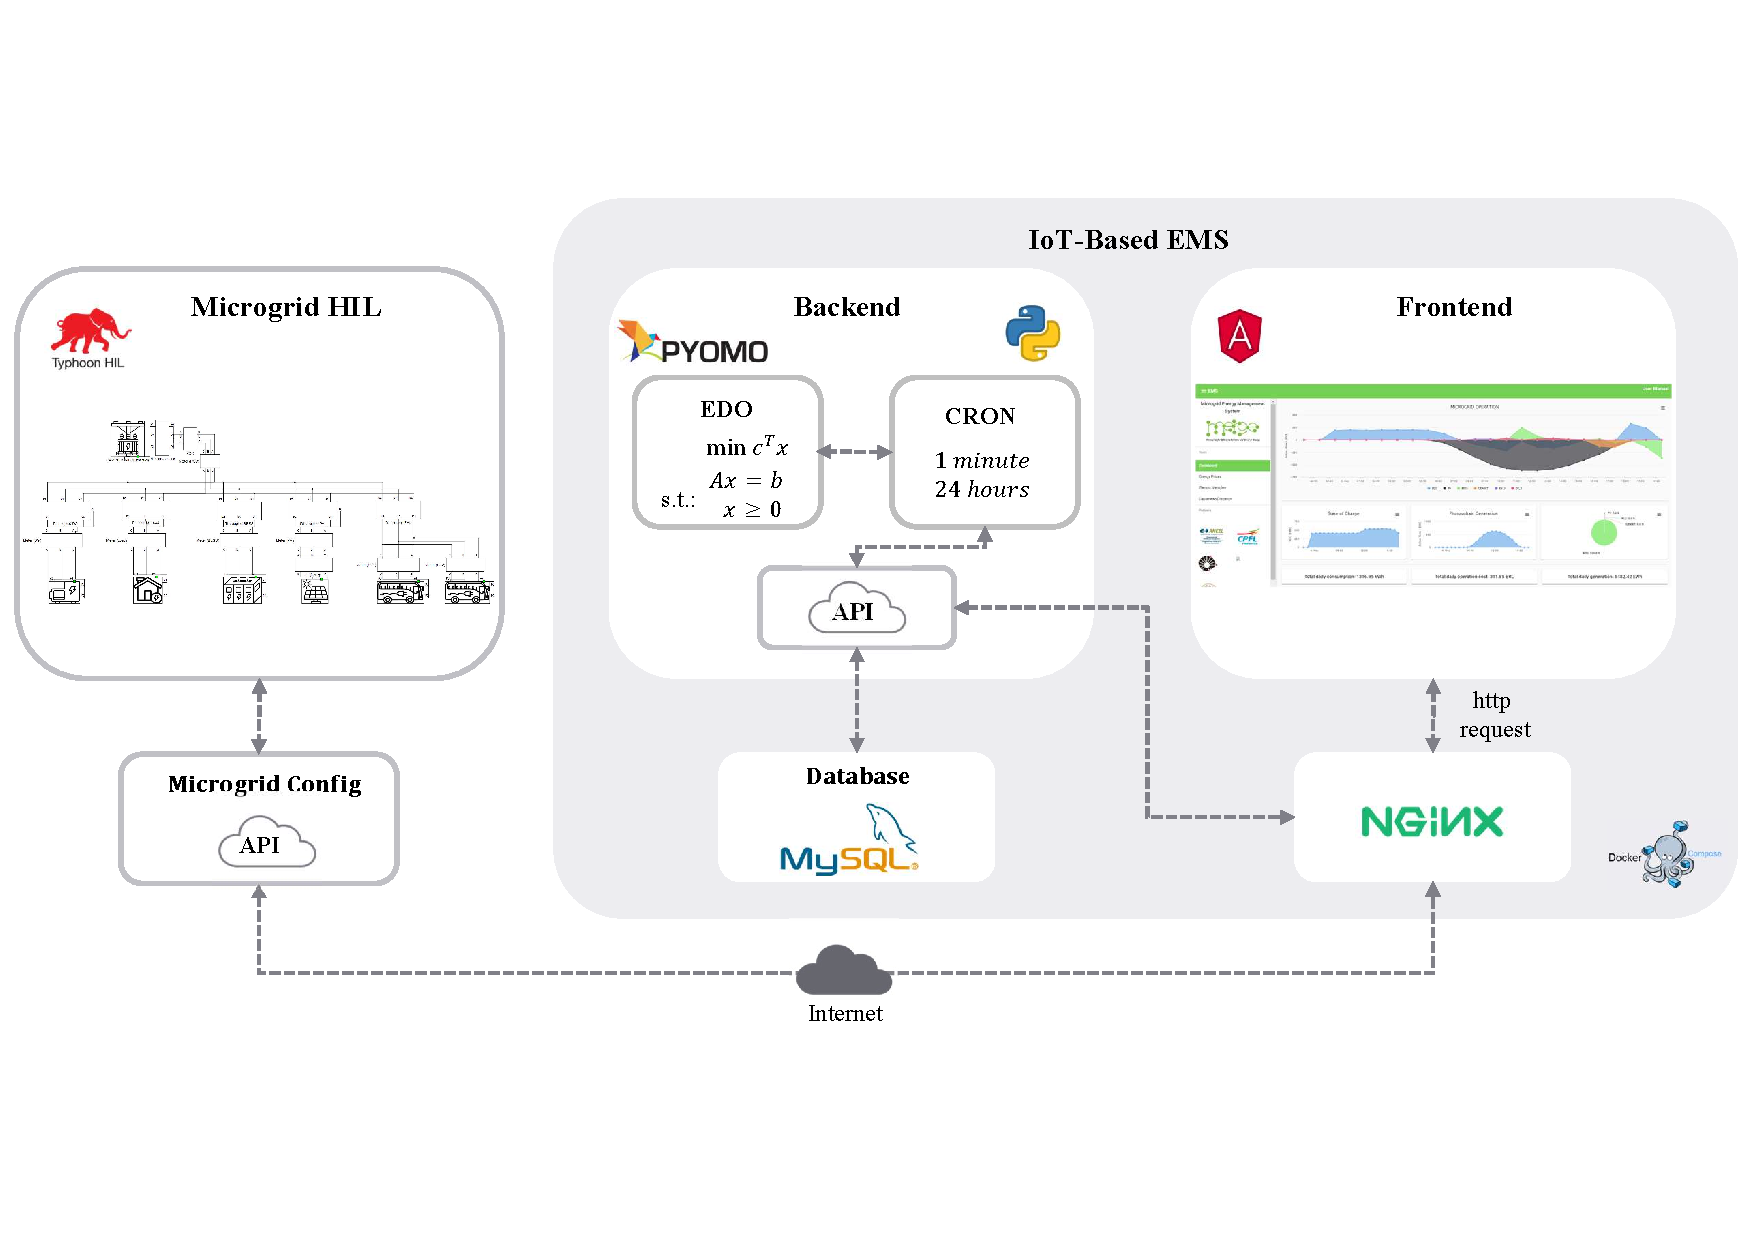
\includegraphics[width=\textwidth]{Figures/ems_architecture.pdf}
    \caption{IoT-based EMS for microgrids software architecture.}
    \label{fig:EMS_Architecture}
\end{figure*}

\subsubsection{Economic Dispatch Optimizer (EDO)}

The main objective of the \gls{edo} module is to 
define the optimal day-ahead scheduling of \gls{der} in the microgrid, 
including the charging and discharging of the \gls{bess}, \gls{pv}
and load curtailment, \gls{genset} dispatch, and \glspl{ev} charging.

The \gls{moop} mentioned in Section \ref{subsec:moop} is solved using the
the solver Cbc \cite{cbc}. The \gls{edo} module is implemented in 
Python using the \gls{pyomo} library \cite{bookpyomo, artpyomo}.

The \gls{edo} module is triggered by the Cron module every 24 hours to
calculate the optimal dispatch for the next day. The results are stored in the
MySQL database and sent to the microgrid controllers via the SIL-API.

The AC \gls{opf} for three-phase unbalanced microgrids is 
modeled as a \gls{milp} problem. The \gls{moop} is solved using the
$\varepsilon$-constraint method, where the first objective function minimizes 
operating costs by considering the cost of electricity from the main grid, 
genset operation, and load/PV curtailment. The second objective function 
(\gls{ens} for \glspl{ev}) is constrained. 
The rest of constraints include power balance, voltage magnitudes, 
current limits, security constraints, genset operation, \gls{bess}
operation and \gls{ev} charging.

\subsubsection{Database}

Measured data during microgrid operation, such as nodal voltages, 
branch currents, power flows, and power injections are stored in a MySQL 
\cite{mysql} database. MySQL is an open-source relational database management 
system, where the user defines the schema, organizes data into tables, 
and sets rules for relationships between tables.

The proposed database structure is related data into seven tables:

\textbf{economic\_dispatch}: Stores dispatch data for the \gls{bess}, 
\gls{pv} and load curtailment, genset dispatch and \glspl{ev} charging.

\textbf{ev\_parameters}: Contains information on electric vehicles, 
including arrival and departure times, charging power, and battery capacity.

\textbf{milp\_parameters}: Contains input parameters for the EDO, 
such as voltage limits, grid power purchase costs, load curtailment costs, 
and genset operational costs.

\textbf{node\_information}: Stores node details including  name, type of DER, 
apparent power limits, and \gls{soc} limits for the BESS.

\textbf{branch\_information}: Contains branch details like name, initial and 
end nodes, resistance and reactance per phase, and maximum current of the circuit.

\textbf{node\_measurement}: Records nodal voltages, active and reactive 
power injections, and SOC for the BESS node.

\textbf{branch\_measurement}: Stores active and reactive power flow values 
and current in the branches.

The \textbf{node\_information} table has an one-to-one relationship with 
the \textbf{branch\_information} table and an one-to-many relationship with 
the \textbf{node\_measurement} table. The \textbf{branch\_information} 
table also has an one-to-many relationship with the \textbf{branch\_measurement} table.

\subsubsection{EMS API}

The \gls{ems} \gls{api} acts as a connector between the backend and frontend, 
facilitating communication and integration. Implemented using Flask, a Python 
web application framework \cite{flask}, it enables interaction between different parts of 
the system. 

Swagger, a tool for \gls{api} maintenance, provides a user-friendly interface 
for testing APIs and visualizing resources. Endpoints such as 
\texttt{/v1/api/ev\_information/} are defined within the 
\gls{ems} \gls{api}, allowing interactions through methods like GET, POST, PUT, 
and DELETE. These endpoints specify the locations where specific actions can 
be performed within the system.

\begin{figure}[!ht]
    \centering
    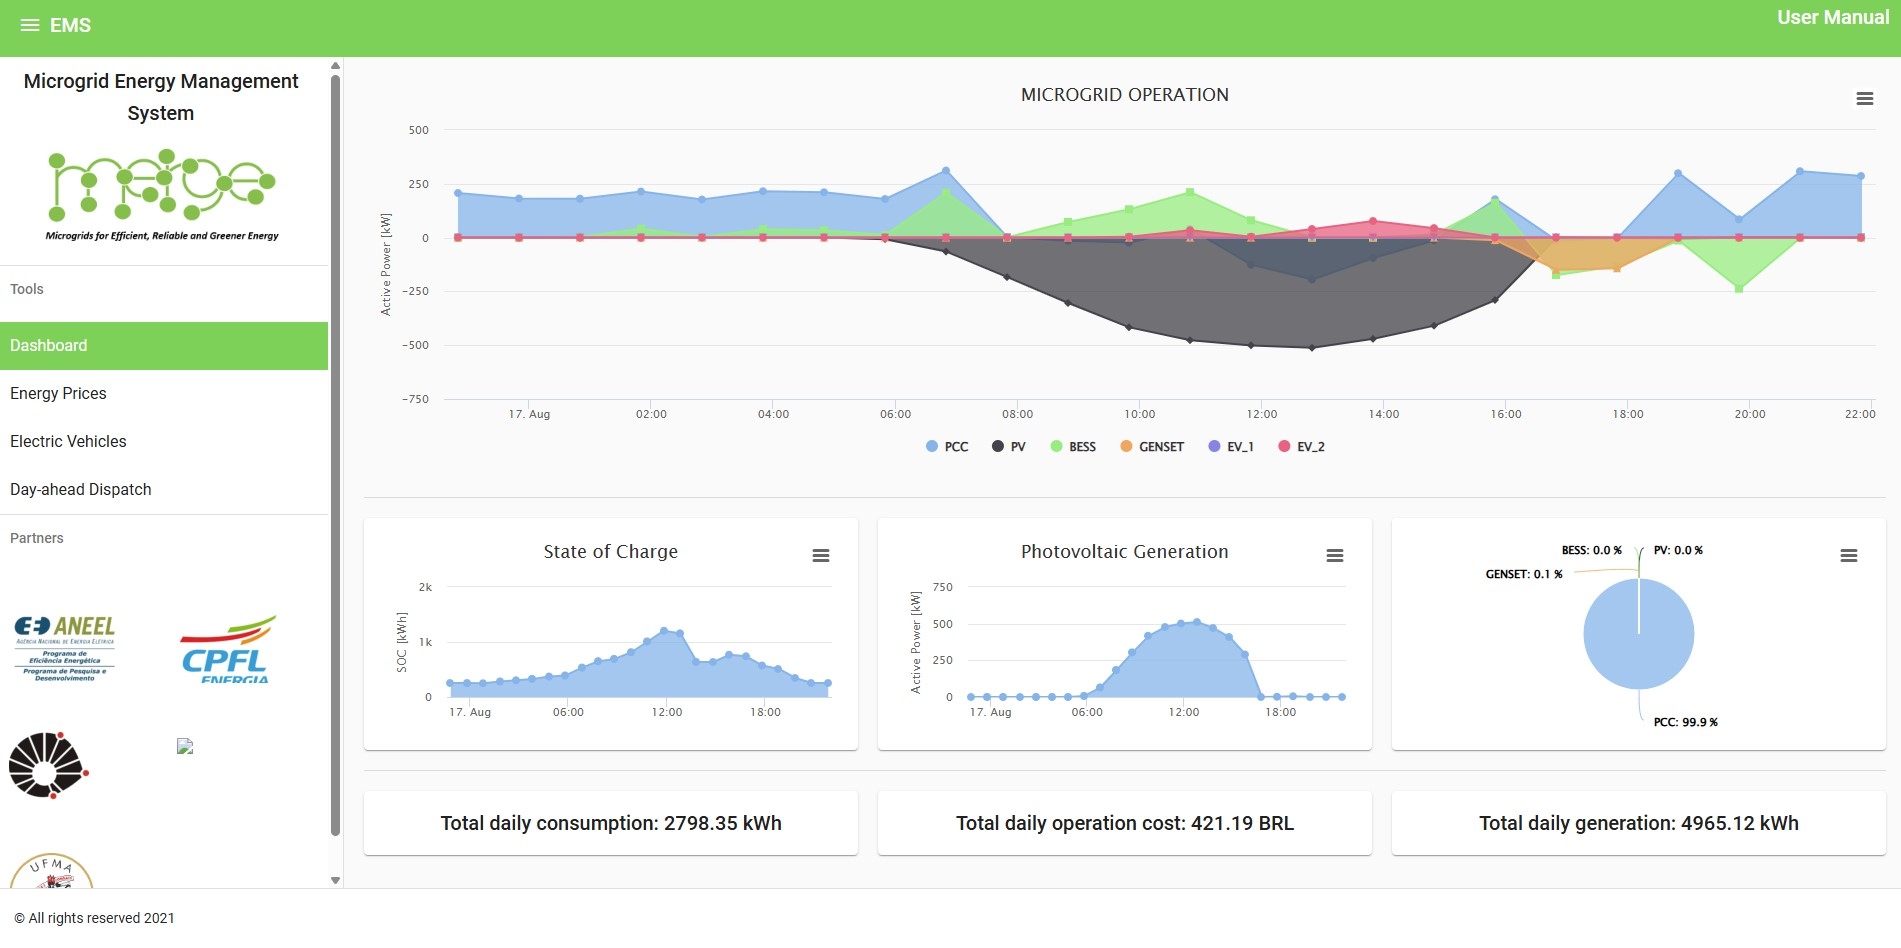
\includegraphics[width=0.48\textwidth]{Figures/EMS/dashboard.jpg}
    \caption{GUI of the EMS Frontend.}
    \label{fig:EMS_Frontend}
\end{figure}

\begin{figure}[!ht]
    \centering
    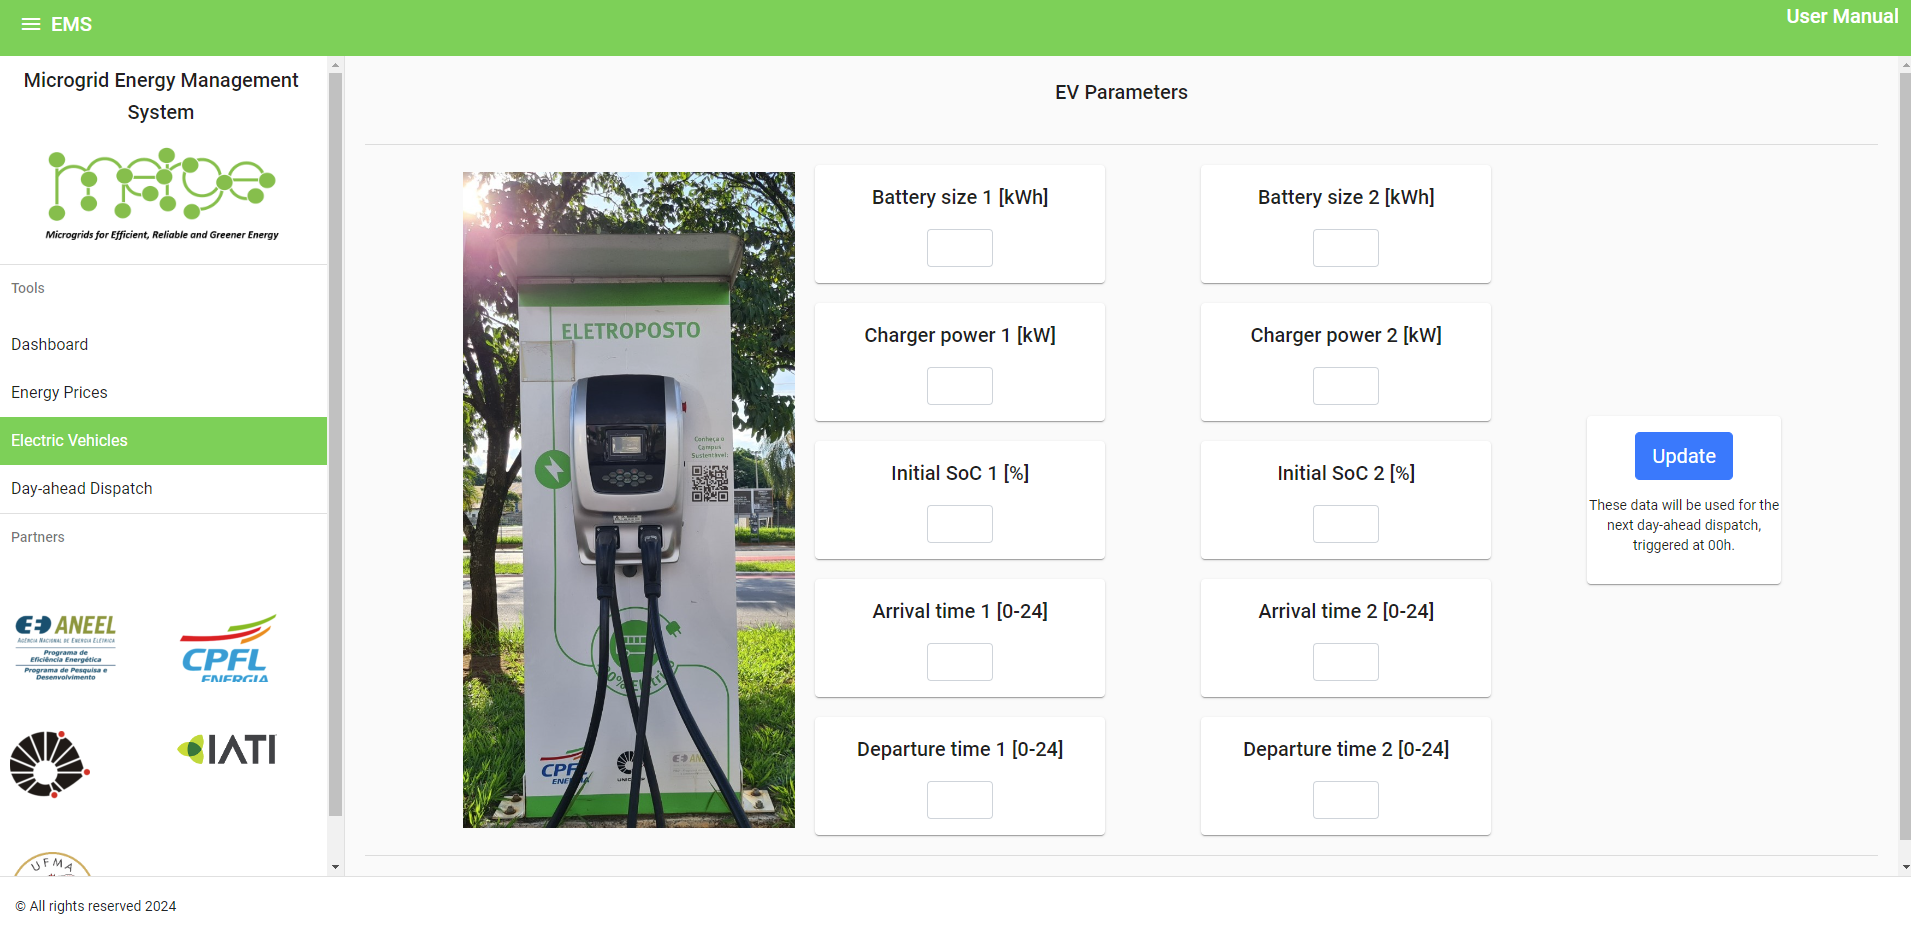
\includegraphics[width=0.48\textwidth]{Figures/EMS/EVs.png}
    \caption{GUI of the EMS Frontend - EV tab.}
    \label{fig:EMS_Frontend_ev}
\end{figure}

\begin{figure*}[!ht]
    \centering
    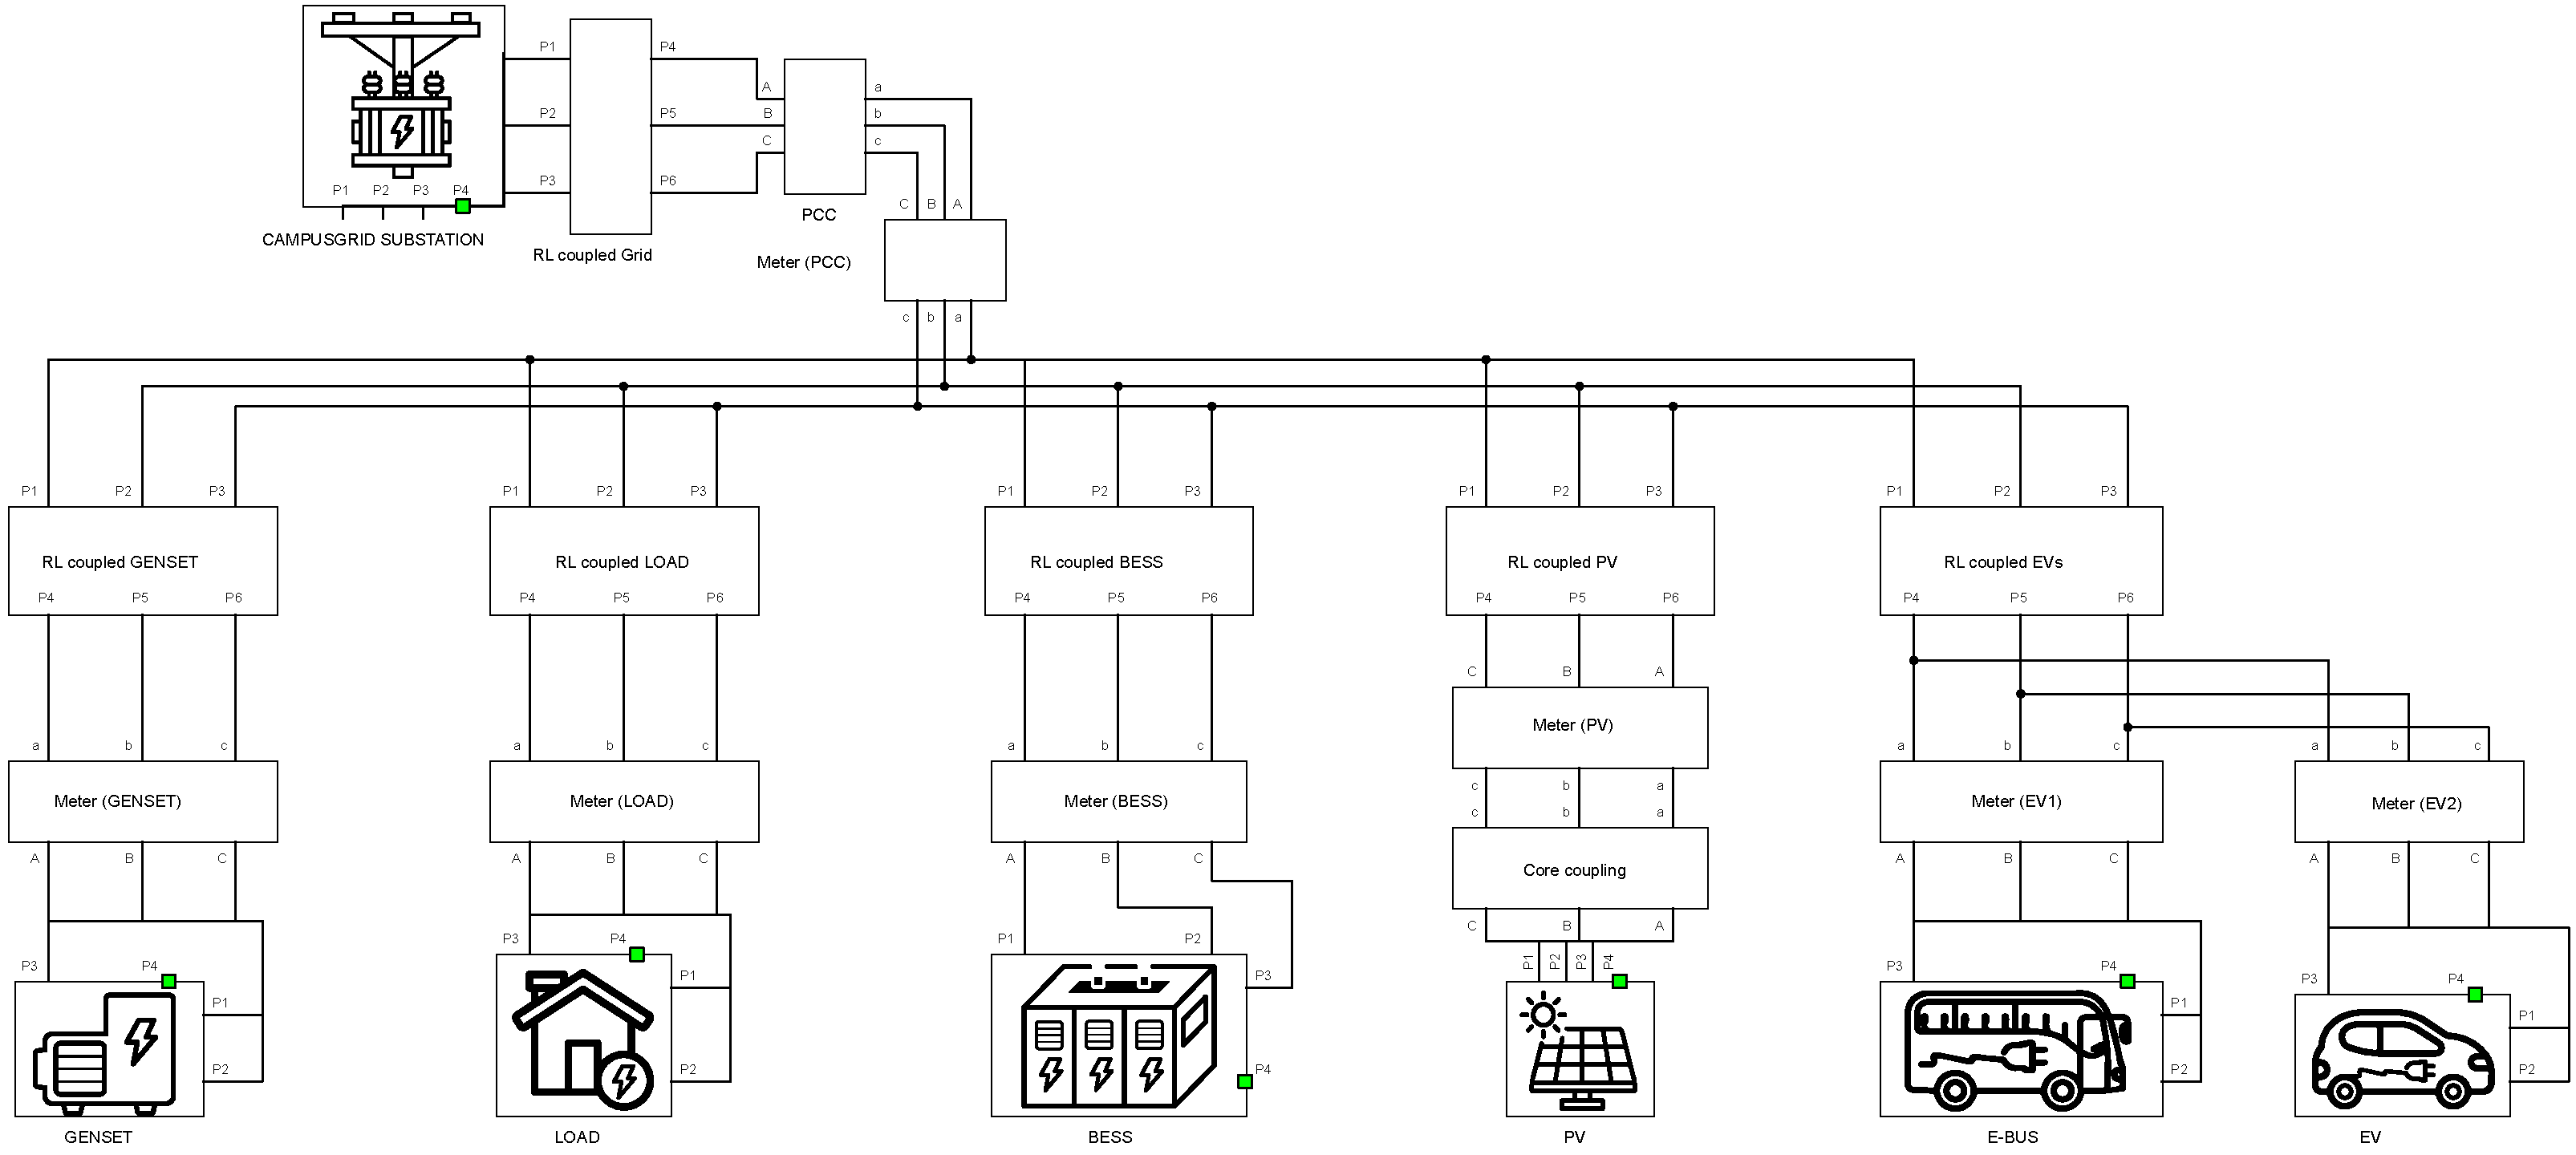
\includegraphics[width=0.98\textwidth]{Figures/schematic_HIL.pdf}
    \caption{Microgrid CAMPUSGRID schematic in Typhoon HIL 604.}
    \label{fig:Microgrid_Schematic}
\end{figure*}

\subsubsection{SIL-API}

In the IoT-based EMS, integration with a simulated microgrid in 
Typhoon HIL \cite{typhoonhil_software} was achieved through the SIL-API 
module \cite{typhoonhil_api}. Typhoon HIL allows real-time simulation 
of microgrids with controllers, controllable via Python scripts.
It consists of three components: Microgrid Config, Data Logger, and an 
\gls{api}.

The Microgrid Config component controls the simulation process, adjusts 
simulation status based on dispatch from the \gls{edo}, and collects real-time 
measurements. Data is logged every minute. The \gls{api}, built with Flask, 
integrates Microgrid Config with the \gls{ems}, providing access to the 
Data Logger records.

Using the REST architectural style, communication between the microgrid 
interface and the EMS is independent, ensuring reliability and fast performance. 
The EMS can be used with various microgrid types, real or simulated, 
as long as both sides support REST communication.

\subsection{Frontend}

The frontend of the IoT-based EMS is a user-friendly \gls{gui} that allows 
users to interact with the application through a web browser. 
It was developed using Angular \cite{angular}, an open-source software that 
uses Typescript as its main programming language.

The GUI includes several tabs, each designed to offer specific functionalities. 
Notably, the \glspl{ev} tab stands out as it was specifically 
developed for this work. Fig. \ref{fig:EMS_Frontend} shows the \gls{gui} of 
the Frontend. The available tabs are:

\begin{itemize}
    \item \text{Dashboard}: The home screen displays real-time microgrid 
    operation data, including SOC of the BESS, PV power generation, and a pie 
    chart comparing energy sources. Daily consumption, operation cost, and 
    generation are also shown.
    \item \text{Electrical Vehicles}: Provides information on 
    arrival and departure times, power charging, and battery capacity for 
    \glspl{ev}, Fig. \ref{fig:EMS_Frontend_ev} shows the new \gls{ev} tab.
    \item \text{Energy Prices}: Users can configure hourly energy prices, 
    thermal generation (genset) costs, and load shedding costs. 
    Configured prices are sent to the database, and a graph displays the 
    changes. For this work, the energy prices were set by \cite{aneel}.
    \item \text{Day-ahead Dispatch}: Shows the dispatch defined by the EDO 
    module for the next day. It includes BESS charge/discharge, load and PV 
    curtailment, and genset dispatch.
\end{itemize}

\section{Case Study}\label{sec:case_study}

The microgrid was modeled using the schematic editor of
Typhoon HIL 604 software \cite{typhoonhil_software}, with data from a real 
three-phase AC microgrid deployed on the campus of \gls{unicamp}, 
São Paulo, Brazil. See Fig. \ref{fig:Microgrid_Schematic}. The model
includes three-phase impedances and meters for each node. The final node is 
equipped with an \gls{ev} charging station, capable of charging one or two 
\glspl{ev} simultaneously. The remaining microgrid parameters are 
detailed in Table \ref{tab:microgrid_parameters}.

\begin{table}[!hb]
    \caption{Microgrid parameters.}
    \label{tab:microgrid_parameters} 
    \vspace{-15pt}
    \begin{center}
        \begin{threeparttable}
            \begin{tabular}{cccc}
            \hline
            Device & Parameter & Magnitude & Unit\\
            \hline
            \multirow{7}{*}{Grid}
            &$\overline{{V}_{i}}$, $\underline{{V}_{i}}$ 
                &\multicolumn{1}{l}{1.05 \quad 0.95} & [kVA]\\
            &${S}^{\text{sub}}$ & 2375 & [\%]\\
            &$\overline{{I}^{\text{PCC}}}$ & 1000 & [A]\\
            &${V}^{nom}$ & 11.9 & [kW]\\
            &${P}^{\text{D}}_{i}$ & 371 & [kW]\\
            &${Q}^{\text{D}}_{i}$ & 260 & [kW]\\
            &${P}^{\text{PV}}_{i}$ & 736 & [kWp]\\
            
            \hline
            
            \multirow{3}{*}{Genset}
            &$\overline{{P}^{\text{G}}_{n}}$, $\underline{{P}^{\text{G}}_{n}}$ 
                &\multicolumn{1}{l}{150 \quad 0} & [kW]\\
            &$\overline{{Q}^{\text{G}}_{n}}$ , $\underline{{Q}^{\text{G}}_{n}}$
                &\multicolumn{1}{l}{150 \quad -150}&[kVAr]\\
            &$\alpha_{n}^{\text{G}}$ &30&[m.u.]\\
            \hline
            \multirow{4}{*}{BESS}
            &$\overline{{P}^{\text{B}}_{m}}$, $\underline{{E}^{\text{B}}_{m}}$ 
                &\multicolumn{1}{l}{1275 \quad 260} & [kWh]\\
            &$\eta^{\text{B}}$ &95&[\%]\\
            &${E}^{\text{B}_{\circ}}_{m}$ &260&[kWh]\\
            &$\overline{{P}^{\text{B}}_{m}}$ &1000&[kW]\\
            \hline
            \multirow{4}{*}{EV}
            &$\overline{{E}^{\text{EV}}_{r}}$, $\underline{{E}^{\text{EV}}_{r}}$ 
                &\multicolumn{1}{l}{324 \quad 64.8} & [kWh]\\
            &$\eta^{\text{EV}}$ & 95 & [\%]\\
            &${E}^{\text{EV}_{\circ}}_{r}$ & 64.8 & [kWh]\\
            &$\overline{{P}^{\text{EV}}_{r}}$ & 80 & [kW]\\
            \hline
            \end{tabular}
        \end{threeparttable}
    \end{center}
\end{table}
\vspace{-15pt}

The \gls{ev} charger offer both slow charging (1 plug - 40 kW) and fast 
charging (using 2 plugs, 40 kW each) \cite{zaneti2022}. For this study, 
fast charging is considered. The arrival and departure times ($t_a$, $t_d$) 
at the charging station are set as 1:00 - 7:00 hours for \gls{ev} 1 and 
8:00 - 14:00 hours for \gls{ev} 2.

To assess the EMS effectiveness in various modes, seven cases were studied:

\begin{itemize}
    \item Case I: Without contingencies.
    \item Case II: Contingency at 16:00 hours.
    \item Case III: Contingency at 08:00 hours. 
    \item Case IV: Without contingencies, including \glspl{ev}.
    \item Case V: Contingency at 16:00 hours with \glspl{ev}.
    \item Case VI: Contingency at 08:00 hours with  \glspl{ev}. 
    \item Case VII: Contingencies at 08:00 and 16:00 hours with \glspl{ev}. 

\end{itemize}

To conduct these case studies, the parameters from 
Table \ref{tab:microgrid_parameters} were applied in the backend model and 
the microgrid simulation in 
Typhoon HIL 604. Consequently, the results are also reflected in the GUI.

\section{Tests and Results}\label{sec:tests_results}

\subsection{Multi-objective Analysis}

To address the \gls{moop}, the $\varepsilon$-constraint method was applied.
Using the Algorithm \ref{alg:e_constraint_method}, it obtains the set 
of non-dominated solutions, forming the Pareto front,
as shown in Fig. \ref{fig:pareto_front}. This algorithm considers nine 
scenarios and two contingencies at 08:00 and 16:00 hours, respectively. 
Moreover, the extreme points and the centroid of the Pareto front were 
analyzed in this study.

\begin{algorithm}
    \caption{$\varepsilon$-Constraint Method for \gls{moop}}
    \label{alg:e_constraint_method}
    \SetAlgoLined
    \KwData{Parameters of the \gls{moop}, including scenarios and contingencies}
    \KwResult{Pareto front}
    % \BlankLine
    \textbf{Initialize:} 
    Set of $\varepsilon_{p}$ values\;
    % \BlankLine
    % \While{MOOP problem is feasible}{
    %     \For{$\varepsilon_{p}$ value}{
    %         \textbf{Solve:} {\eqref{final_equation}}\;
    % }}
    % \While{MOOP problem is feasible}{
        \For{each $\varepsilon_{p}$ value in the set}{
            \textbf{Solve:} {\eqref{final_equation}}\;
            \textbf{Store:} Non-dominated solutions\;
    }% }}
    % \BlankLine
    \textbf{Generate} Pareto front\;
    % \textbf{Measure:} Euclidean distance to the ideal point\;
    \textbf{Compute:} The centroid of the Pareto front\;

\end{algorithm}

For each point, the stochastic \gls{edo}
determined one optimal day-ahead dispatch of the \gls{bess} and \glspl{ev} 
for the nine scenarios and two contingencies.
The first extreme point represents the solution with the maximum value 
of $f_{ens}$ and the minimum value of $f_{costs}$, while the second extreme 
point represents the solution with the minimum value of $f_{ens}$ and the
maximum value of $f_{costs}$. The \gls{bess} and \gls{ev} dispatches for 
these two extreme points are illustrated in Fig. \ref{fig:extreme_points}.

The first point, Fig. \ref{fig:first_extreme_point}, 
the \gls{bess} is dispatched without any \gls{ev} charging. This occurs because, 
at this point, $\varepsilon_{p} = 518.4$, which represents the maximum value 
of $f_{ens}$, resulting in no \gls{ev} being charged. Moreover, 
the minimum value of $f_{costs} = 10,926.93$ indicates that no additional 
costs are incurred from charging the \glspl{ev}.

In contrast, at the second extreme point, Fig. \ref{fig:second_extreme_point}, 
shows the dispatch of both, the BESS and \glspl{ev}. In this case, 
$\varepsilon_{p} = 0$ represents the minimum value of $f_{ens}$, 
meaning that both \glspl{ev} are charged to 100\%. 
This point is associated with a maximum value of $f_{costs} = 16,410.89$, 
reflecting the higher costs due to the full charging of the \glspl{ev}. 
In conclusion, higher \gls{ev} charging leads to higher operational costs.

\begin{figure*}[ht!]
    \centering
    \tikzstyle{every pin}=[
    fill=white,
    draw=gray,
    font=\footnotesize]
    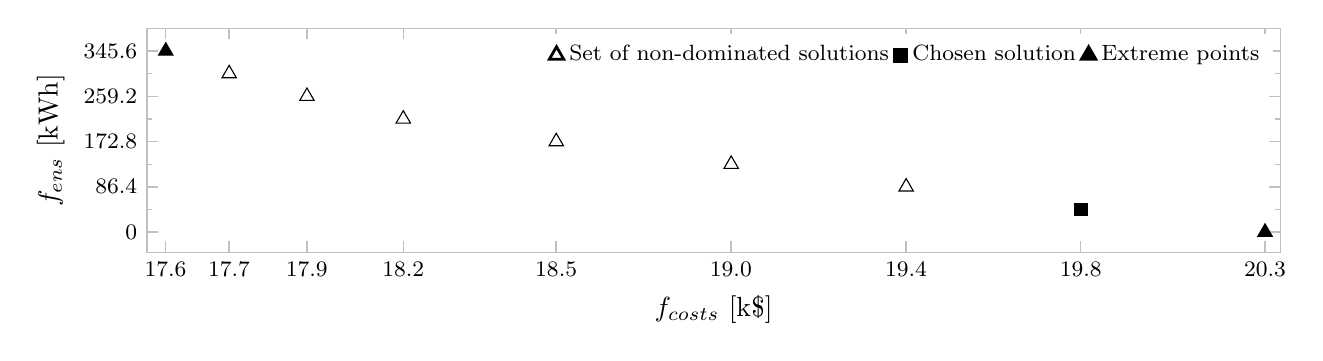
\begin{tikzpicture}
    \begin{axis}[
        %width=240pt,
        % height = 140pt,
        % x dir = reverse,
        y post scale = 0.5,
        x post scale = 2.1,
        xlabel={$f_{costs}$ [k\$]},
        xlabel near ticks,
        % axis x line = bottom,
        % axis line shift = 10pt,
        ylabel={$f_{ens}$ [kWh]},
        ylabel near ticks,
        % axis y line = left,
        % axis line style={|-stealth},
        % axis x discontinuity=crunch,
        tick style = {line width = 0.5, color = lightgray, 
            major tick length=4pt,minor tick length=2pt, 
            minor y tick num =1, xtick = {
            17645, 
            17799,
            17988,
            18222,
            18593,
            19017,
            19442,
            19866,
            20313}
            },
        xticklabels = {
            17.6,
            17.7,
            17.9,
            18.2,
            18.5,
            19.0,
            19.4,
            19.8,
            20.3
            },
        tick label style = {font=\footnotesize, ytick distance=86.4
            },
        xtick align = {inside},
        ytick align = {inside},
        % extra x ticks={10926.93},
        %extra x tick labels={10926.93},
        % label style = {font=\small},
        % legend style = {font=\footnotesize, at={(0.5,1.05)},    
        %     anchor=south, legend cell align=left, line width=0.5pt, 
        %     draw=lightgray, legend columns = 2}
        legend style = {font=\footnotesize, at={(0.995,0.98)},    
            anchor= north east, legend cell align=center, line width=1pt, 
            draw = none, legend columns = 3},
        ymax=388.8,
        xmin=17600, xmax=20350,
        % enlarge x limits=0.05,
        axis line style = {line width = 0.5pt, lightgray},
        scaled ticks=false
        ]

    
     % Set of non-dominated solutions 
    \addplot[mark = triangle, only marks, mark size = 3pt,
    black] 
    coordinates {

        (17799.57	,302.4)
        (17988.30	,259.2)
        (18222.13	,216)
        (18593.29	,172.8)
        (19017.81	,129.6)
        (19442.34	,86.4)
        % (19866.86	,43.2)
              
        };
    \addlegendentry{Set of non-dominated solutions}
    
    % Centroid
    \addplot [mark size = 2.2pt, only marks, mark = square*]
        coordinates {
        (19866.86	,43.2)
        };
    \addlegendentry{Chosen solution}

    \addplot [mark size = 3pt, only marks, mark = triangle*]
        coordinates {
        (17645.70	,345.6)
        (20313.20	,0)
        };
    \addlegendentry{Extreme points}
    % \node [coordinate, pin=above right:{Centroid}] at
    %     (axis cs: 13863.73, 259.2 ) {};
    % \node [coordinate, pin=above right:{Ideal Point}] at
    %     (axis cs: 10926.93, 0) {};
    \end{axis}
\end{tikzpicture}
    \caption{Pareto front}
    \label{fig:pareto_front}
\end{figure*}

\begin{figure*}[htb!]
    \centering
    \subfloat[Dispatch for the first extreme point]{%
        \input{Figures/5_firs_point.tex}
        \label{fig:first_extreme_point}
    }
    \hfill
    \subfloat[Dispatch for the second extreme point]{%
        \begin{tikzpicture}
    \begin{axis}[ybar stacked,
        xlabel={Period time [h]},
        ylabel={Active power [kW]},
        ylabel near ticks,
        xlabel near ticks,
        bar width=4pt,
        tick style = {line width = 0.5, color = lightgray, 
            major tick length=4pt,minor tick length=2pt,
            minor x tick num = 3, minor y tick num =1},
        tick label style = {font=\footnotesize, xtick distance=4, ytick distance=100,
            xticklabels={01:00, 01:00, 04:00, 08:00, 12:00, 16:00, 20:00 }},
        legend style = {font=\footnotesize, at={(0.99,0.98)}, 
            legend cell align=left, line width=0.5pt, draw=lightgray},
        legend entries={BESS,E-BUS,EV},
        ymin=-350, ymax=250,
        xmin=0, xmax=25,
        axis line style = {lightgray, line width = 0.5pt},
        cycle multi list={
        lightgray, gray, black\nextlist
        fill
        }
        ]

        \addplot table 
        [col sep=comma, x = h, y=P_BESS] {./Data/second_point.dat};
        \addplot table
        [col sep=comma, x = h, y=P_EV_1] {./Data/second_point.dat};
        \addplot table
        [col sep=comma, x = h, y=P_EV_2] {./Data/second_point.dat};
        
    \end{axis}
\end{tikzpicture}
        \label{fig:second_extreme_point}
        }
    \caption{Dispatch of the BESS and EVs for the 
    first and second extreme points.}
    \label{fig:extreme_points}
\end{figure*}

Analyzing the extreme points shows that neither solution favors both objective 
functions. For this reason, the centroid of the Pareto front is calculated, 
representing the best compromise between the two objectives.

Fig. \ref{fig:pareto_front} illustrates this centroid, identified by the pair
of values $f_{ens} = 259.2$ kWh and $f_{costs} = 13 863.73$ \$. This solution 
ensure that at least one \gls{ev} is 
charged to 100\% of its capacity. In this case study, 
the initial \gls{soc} is 64.8 kWh (20\%). By adding 259.2 kWh, is guaranteed 
that the \gls{ev} reaches its total maximum energy capacity of 324 kWh (100\%).

\subsection{Results of Case Studies}

For the following case studies, the centroid of the Pareto front was 
adopted as the $\varepsilon_{p}$ value. This value was used to solve the
\gls{moop} for seven distinct cases. For each case, the stochastic \gls{edo}
determined one optimal day-ahead dispatch of the \gls{bess} and \gls{ev} 
for the nine scenarios. 
The results of the \gls{bess}, genset dispatch, \gls{pv} curtailment, 
and \glspl{ev} are presented in Fig. \ref{fig:bess_dispatch} through 
Fig. \ref{fig:ev_1_2_dispatch}, respectively. 
In addition, the microgrid's 24-hour operation, the \gls{soc} of 
the \gls{bess}, and the \gls{pv} generation are visualized in Figs.
\ref{fig:microgrid_operation}, \ref{fig:soc_operation} and 
\ref{fig:pv_operation} respectively. 

Case I represents the normal operation of the microgrid 
without any contingencies. The optimal dispatch of the \gls{bess} takes 
advantage of the PV generation to charge during the high \gls{pv} and 
discharge during the high energy cost periods.
Fig. \ref{fig:case_I_bess_dispatch} shows the BESS dispatch, while
Fig. \ref{fig:case_I_operation} illustrates the microgrid's 24-hours 
operation. Figs. \ref{fig:case_I_soc} and \ref{fig:case_I_pv_generation} 
display the \gls{soc} of the \gls{bess} and \gls{pv} generation, respectively.

In the second case, the \gls{bess} charged at 01:00 and 13:00 hours, almost
reaching its total capacity, see Fig. \ref{fig:case_II_bess_dispatch} 
and \ref{fig:case_II_operation}. This aimed to prepare for the contingency 
(two hours of duration) and supply the demand along with the \gls{genset} 
dispatch. Before the contingency, \gls{pv} generation supplied the demand. 
During the contingency, there was PV curtailment in the first hour, as 
shown in Fig. \ref{fig:case_II_pv_curt_dispatch}. Although the BESS was 
almost fully charged, during the contingency, the \gls{pv} generation was 
disconnected, and the generator was operated to supply the demand, as the 
BESS dispatch is unique for the nine scenarios of the stochastic analysis. 
This operation is illustrated in Fig. \ref{fig:case_II_operation}.

Unlike the second case, the third case in Fig. \ref{fig:case_III_bess_dispatch} 
shows the charge of the \gls{bess} reached the 25\% of its capacity, 
for discharge during the contingency and supply the demand along with the 
genset dispatch. After the contingency, the \gls{bess} utilizes the 
PV generation to charge and discharge during the high-cost energy periods. 
The operation of the microgrid is shown in Fig. \ref{fig:case_III_operation}.

Cases II and III are similar and present one contingency at 16:00 
and 08:00 hours, respectively. Both cases shows genset dispatch and PV 
curtailment, as shown in Figs. \ref{fig:genset_genset_dispatch} 
and \ref{fig:pv_curtailment_dispatch}. It is important to mention that 
during the contingency, the \gls{bess} act like grid forming, controlling 
the voltage and frequency of the microgrid. 

Case IV, similar to the first case, shows the operation of the microgrid 
without contingencies but includes \glspl{ev}. 
Using $\varepsilon_{p} = 259.2$ and 
considering the arrival and departure times of the \glspl{ev} from Section
\ref{sec:case_study}, the \gls{edo} dispatched only one \gls{ev}, in 
this case, the second \gls{ev}, as shown in 
Fig. \ref{fig:case_IV_ev_dispatch}. The \gls{edo} prioritizes 
this \gls{ev} because it can take advantage of the solar energy 
available during the day, reaching a \gls{ens} equal to $0$ (100\%). 
The operation of the microgrid, \gls{soc} of 
the \gls{bess} and \gls{pv} operation is illustrated in 
Figs. \ref{fig:case_IV_operation}, \ref{fig:case_IV_soc} 
and \ref{fig:case_IV_pv_generation} respectively.

The fifth and sixth cases are similar to the second and third cases but with 
the inclusion of \glspl{ev}. The \gls{bess} dispatch, genset and 
\gls{pv} curtailment for cases V and VI are shown in 
Figs. \ref{fig:case_V_bess_dispatch}, \ref{fig:case_VI_bess_dispatch}, 
\ref{fig:case_V_genset_dispatch}, \ref{fig:case_VI_genset_dispatch}, 
\ref{fig:case_V_pv_curt_dispatch} and \ref{fig:case_VI_pv_curt_dispatch}, 
respectively. The analysis of the
second and third cases for the genset dispatch and \gls{pv} curtailment is 
valid for the fifth and sixth cases. The operation of the microgrid, 
\gls{soc} of the \gls{bess} and \gls{pv} operation is shown in 
Figs. \ref{fig:case_V_operation}, \ref{fig:case_VI_operation}, 
\ref{fig:case_V_soc}, \ref{fig:case_VI_soc}, \ref{fig:case_V_pv_generation}
and \ref{fig:case_VI_pv_generation} respectively.

The \gls{edo} determined that one \gls{ev} charge in cases IV and V, even 
though both \glspl{ev} were included in these scenarios. However, it is 
important to note that in case VI, the \gls{edo} determined 
the charge both \glspl{ev}. Regarding the \gls{ens}, both EVs reached 50\% 
of their charge, indicating that the \gls{edo} can charge either one or 
both EVs. This occurs because the centroid ($\epsilon = 259$) was adopted.

Case VII, includes two contingencies at 08:00 and 16:00 hours, respectively. 
The \gls{bess} dispatch, genset and \gls{pv} curtailment are shown in
Figs. \ref{fig:case_VII_bess_dispatch}, \ref{fig:case_VII_genset_dispatch},
and \ref{fig:case_VII_pv_curtailment}, respectively. The operation of the
microgrid is illustrated in Fig. \ref{fig:case_VII_operation}. 

The demand for the first contingency was supplied by the \gls{bess} and
\gls{pv} generation, while the second contingency was supplied by the
\gls{bess} and the \gls{genset}, there was \gls{pv} curtailment 
to maintain the power balance. In contrast to the 
Fig. \ref{fig:second_extreme_point}, where both \glspl{ev} was charged,
in this case, only one \gls{ev} was charged, as shown 
in Fig. \ref{fig:case_VII_ev_2_dispatch}, this is due to the
$\varepsilon_{p}$ value adopted in the \gls{edo} that charge at least one
\gls{ev} to 100\% of its capacity.

In summary, in grid-connected operations without contingencies 
(Case I and Case IV), the BESS charges during the day, leveraging solar 
energy when costs are lower. Contingencies in Cases II, III, V, VI and VII, 
the BESS presents a single optimal operation defined in the face of a 
stochastic analysis, it is possible to observe that in cases where there was 
a contingency, it was more economically advantageous to dispatch 
the \gls{genset} and perform \gls{pv} curtailment the demand in these rare 
moments and leave the BESS prepared for discharge in peak periods.

\begin{figure*}[!htb]
    \centering
    \subfloat[Case I: Without contingencies.]{
        \includegraphics[width=0.45\textwidth]{Figures/1_case/bess-dispatch.pdf}
        \label{fig:case_I_bess_dispatch}
    }
    \subfloat[Case II: Contingency at 16:00 hours.]{
        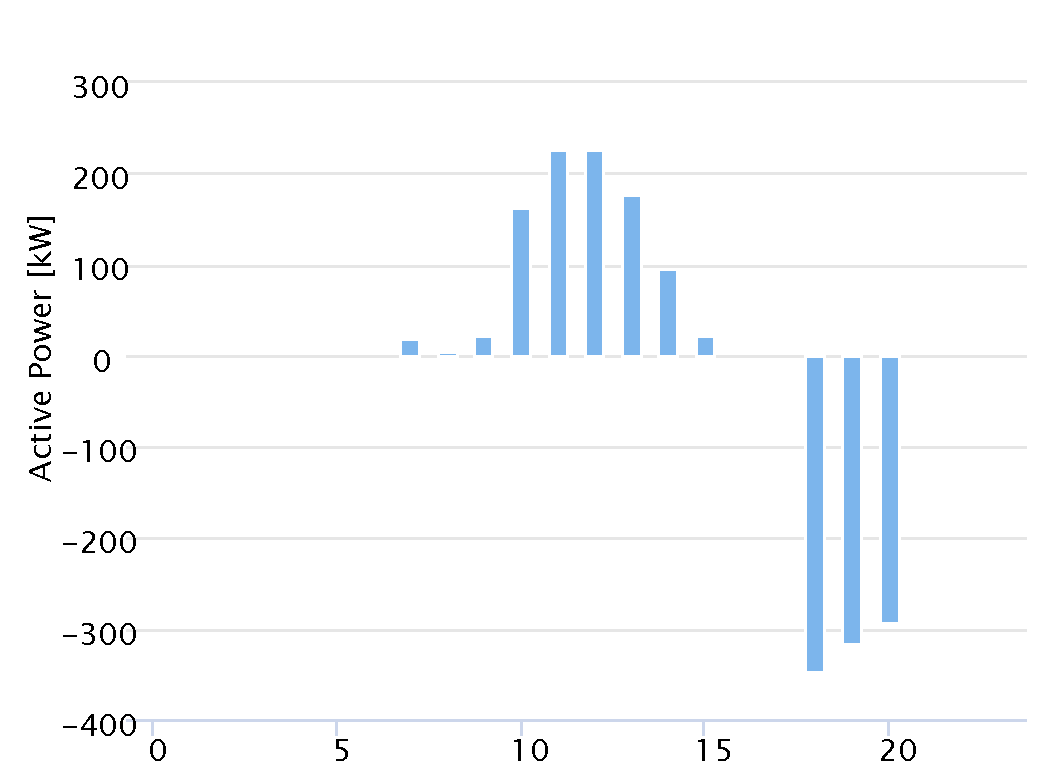
\includegraphics[width=0.45\textwidth]{Figures/2_case/bess-dispatch.pdf}
        \label{fig:case_II_bess_dispatch}
    }
    \vfill
    \subfloat[Case III: Contingency at 08:00 hours.]{
        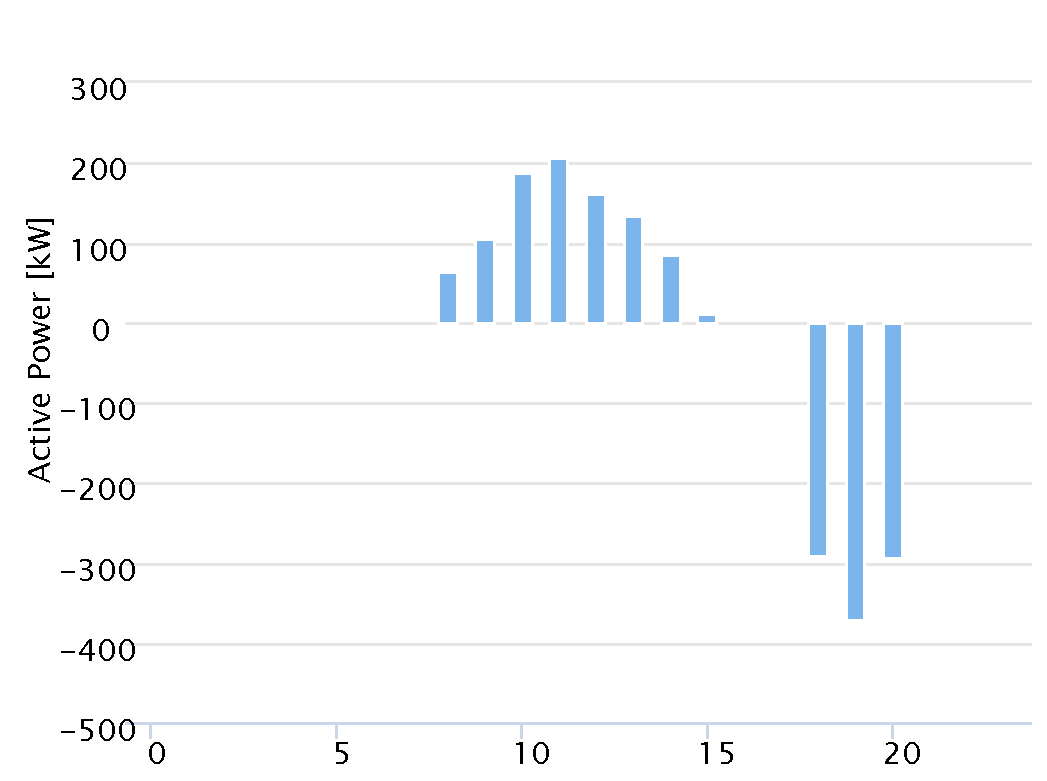
\includegraphics[width=0.45\textwidth]{Figures/3_case/bess-dispatch.pdf}
        \label{fig:case_III_bess_dispatch}
    }
    \subfloat[Case IV: Without contingencies, including \glspl{ev}.]{
        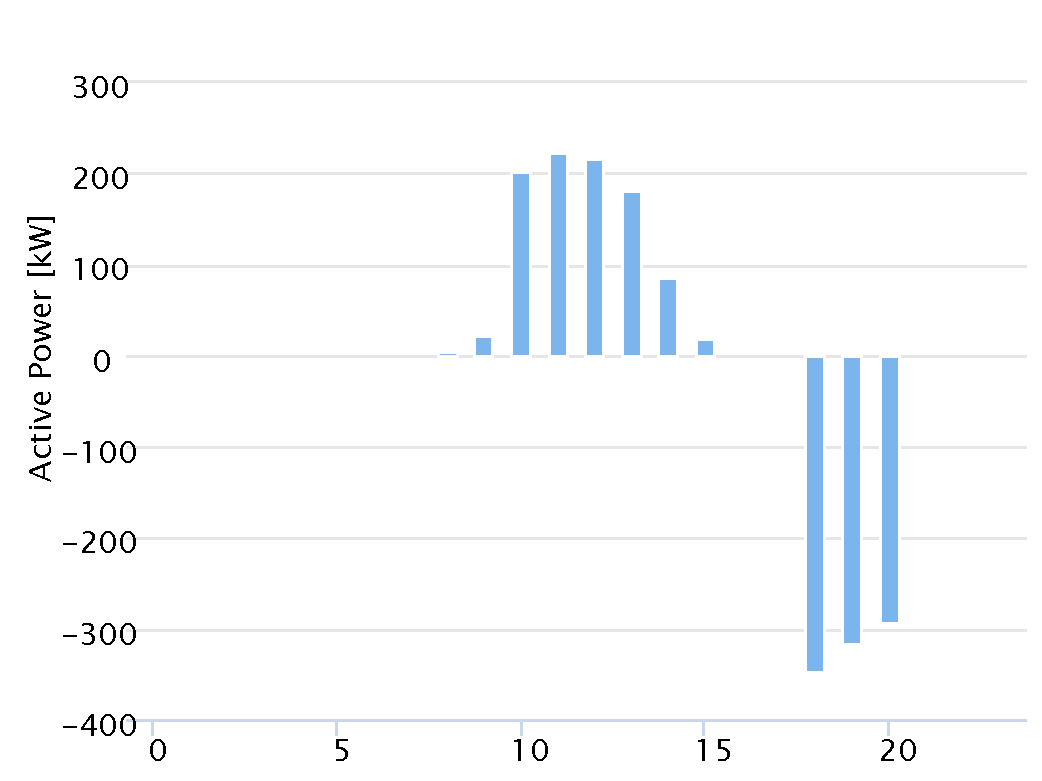
\includegraphics[width=0.45\textwidth]{Figures/4_case/bess-dispatch.pdf}
        \label{fig:case_IV_bess_dispatch}
    }
    \vfill
    \subfloat[Case V: Contingency at 16:00 hours with \glspl{ev}.]{
        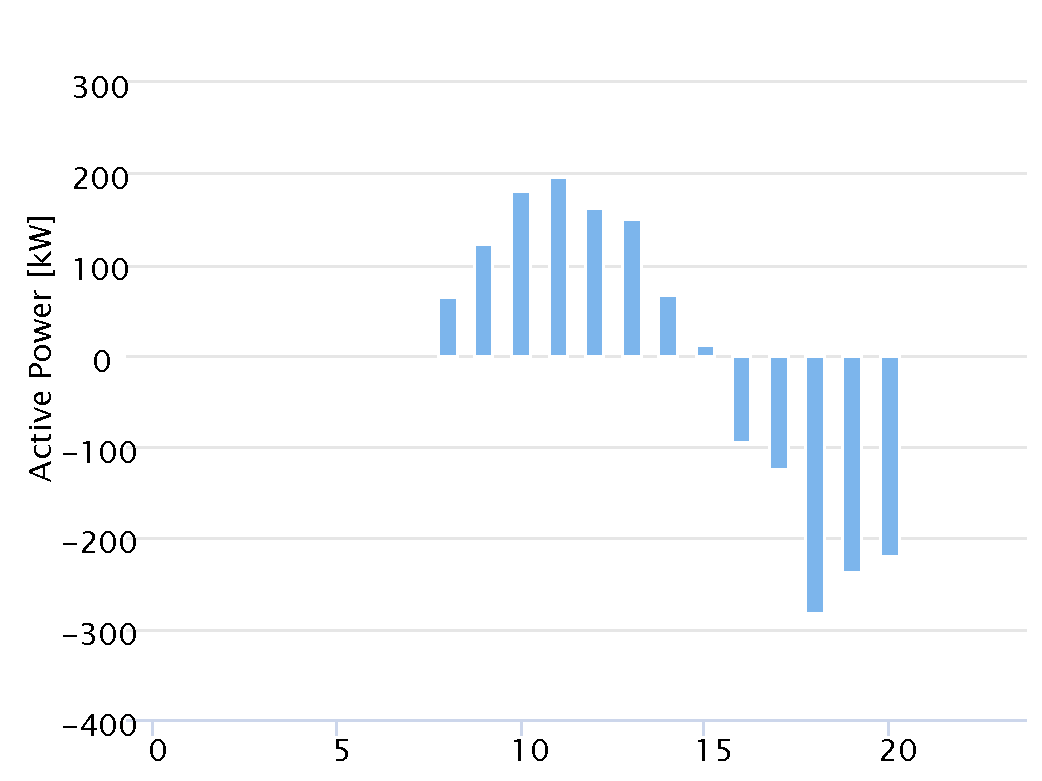
\includegraphics[width=0.45\textwidth]{Figures/5_case/bess-dispatch.pdf}
        \label{fig:case_V_bess_dispatch}
    }
    \subfloat[Case VI: Contingency at 08:00 hours with \glspl{ev}.]{
        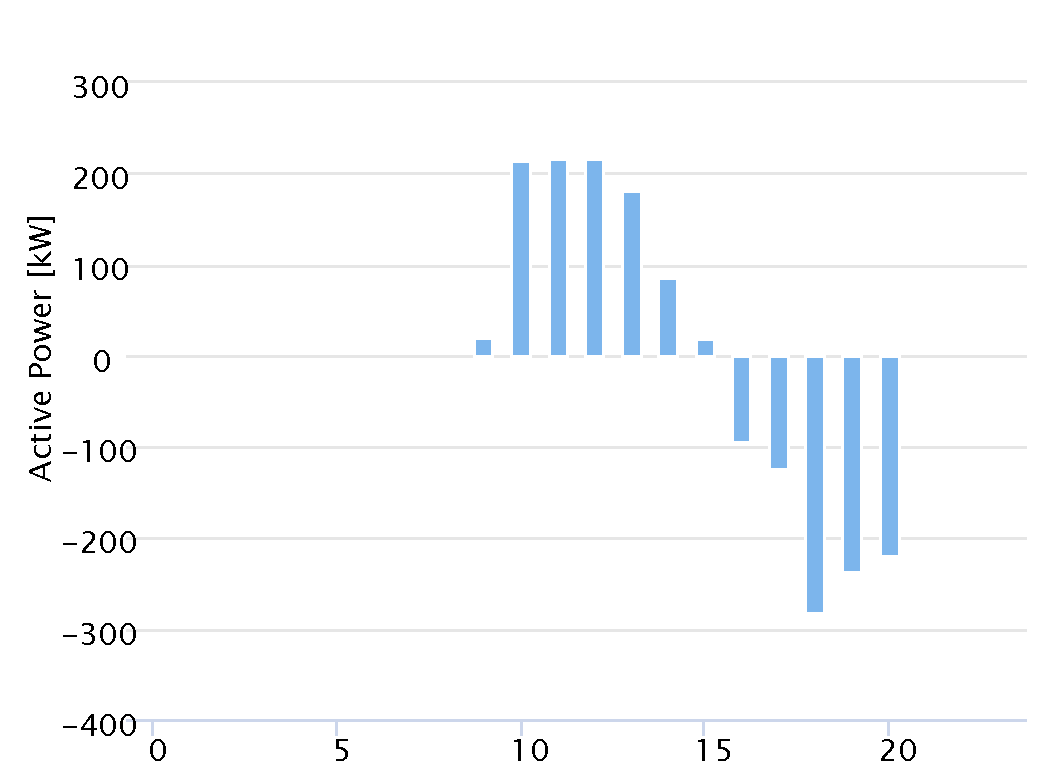
\includegraphics[width=0.45\textwidth]{Figures/6_case/bess-dispatch.pdf}
        \label{fig:case_VI_bess_dispatch}
    }
    \caption{BESS dispatch for each case.}
    \label{fig:bess_dispatch}
\end{figure*}

\begin{figure*}[!htb]
    \centering
    \subfloat[Case II: Contingency at 16:00 hours.]{
        \includegraphics[width=0.45\textwidth]{Figures/2_case/genset-dispatch.pdf}
        \label{fig:case_II_genset_dispatch}
    }
    \subfloat[Case III: Contingency at 08:00 hours.]{
        \includegraphics[width=0.45\textwidth]{Figures/3_case/genset-dispatch.pdf}
        \label{fig:case_III_genset_dispatch}
    }
    \vfill
    \subfloat[Case V: Contingency at 16:00 hours with \glspl{ev}.]{
        \includegraphics[width=0.45\textwidth]{Figures/5_case/genset-dispatch.pdf}
        \label{fig:case_V_genset_dispatch}
    }
    \subfloat[Case VI: Contingency at 08:00 hours with \glspl{ev}.]{
        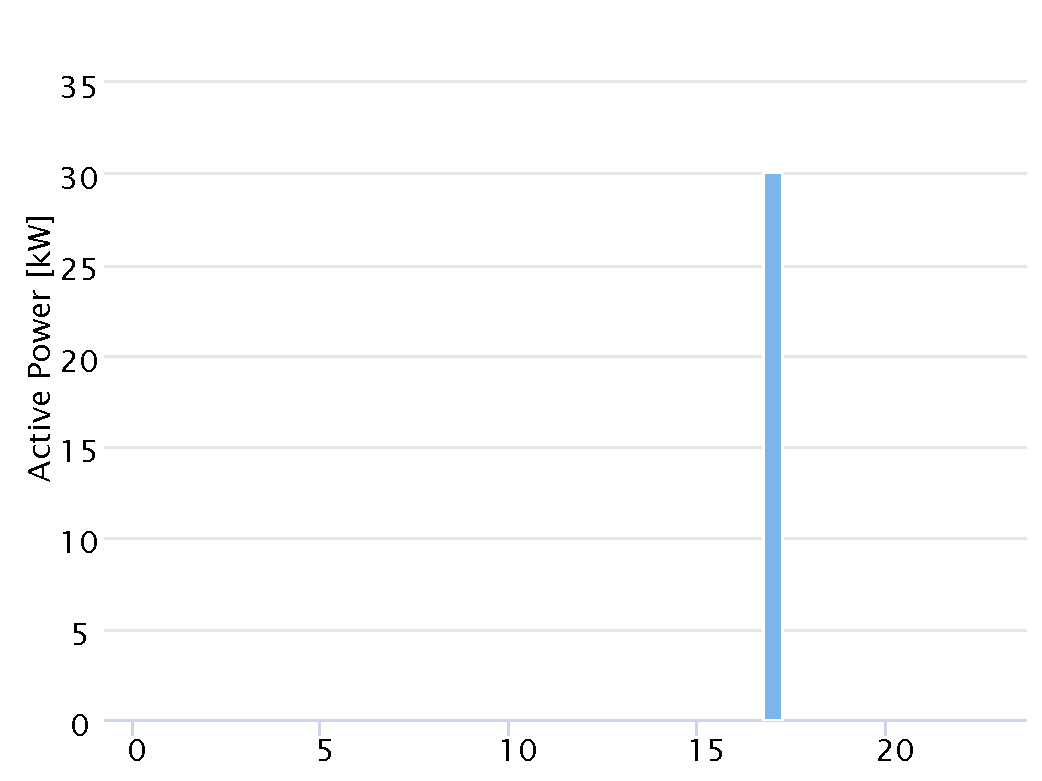
\includegraphics[width=0.45\textwidth]{Figures/6_case/genset-dispatch.pdf}
        \label{fig:case_VI_genset_dispatch}
    }
    \caption{Genset dispatch for each case.}
    \label{fig:genset_genset_dispatch}
\end{figure*}

\begin{figure*}[!htb]
    \centering
    \subfloat[Case II: Contingency at 16:00 hours.]{
        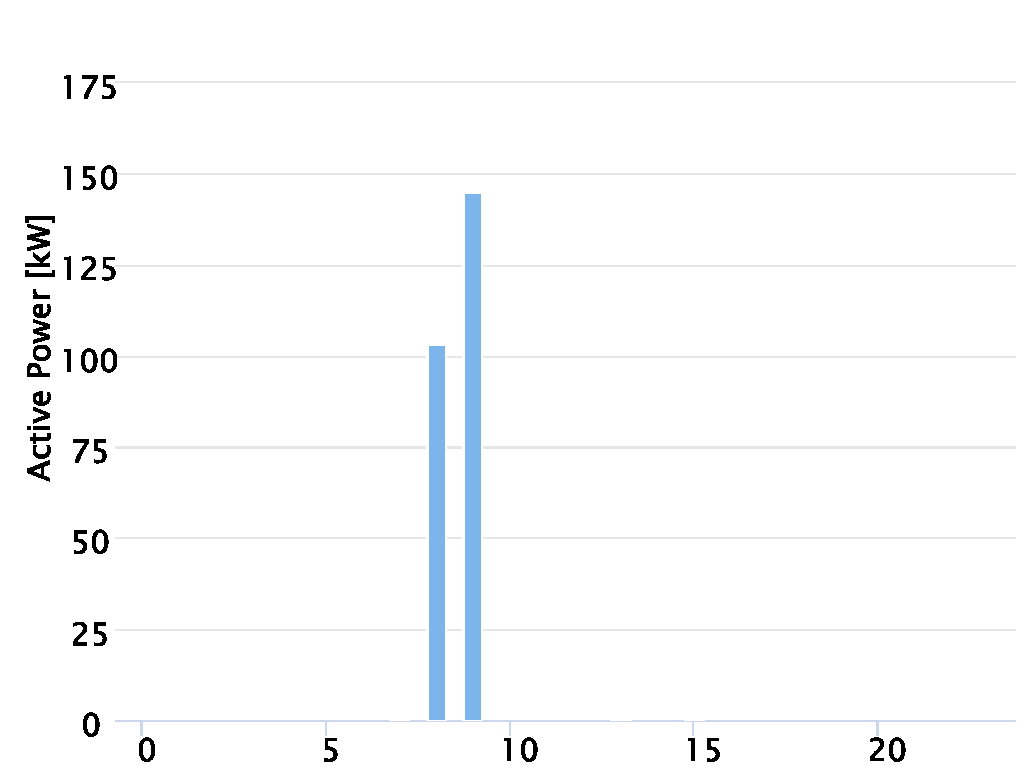
\includegraphics[width=0.45\textwidth]{Figures/2_case/pv-curtailment.pdf}
        \label{fig:case_II_pv_curt_dispatch}
    }
    \subfloat[Case III: Contingency at 08:00 hours.]{
        \includegraphics[width=0.45\textwidth]{Figures/3_case/pv-curtailment.pdf}
        \label{fig:case_III_pv_curt_dispatch}
    }
    \vfill
    \subfloat[Case V: Contingency at 16:00 hours with \glspl{ev}.]{
        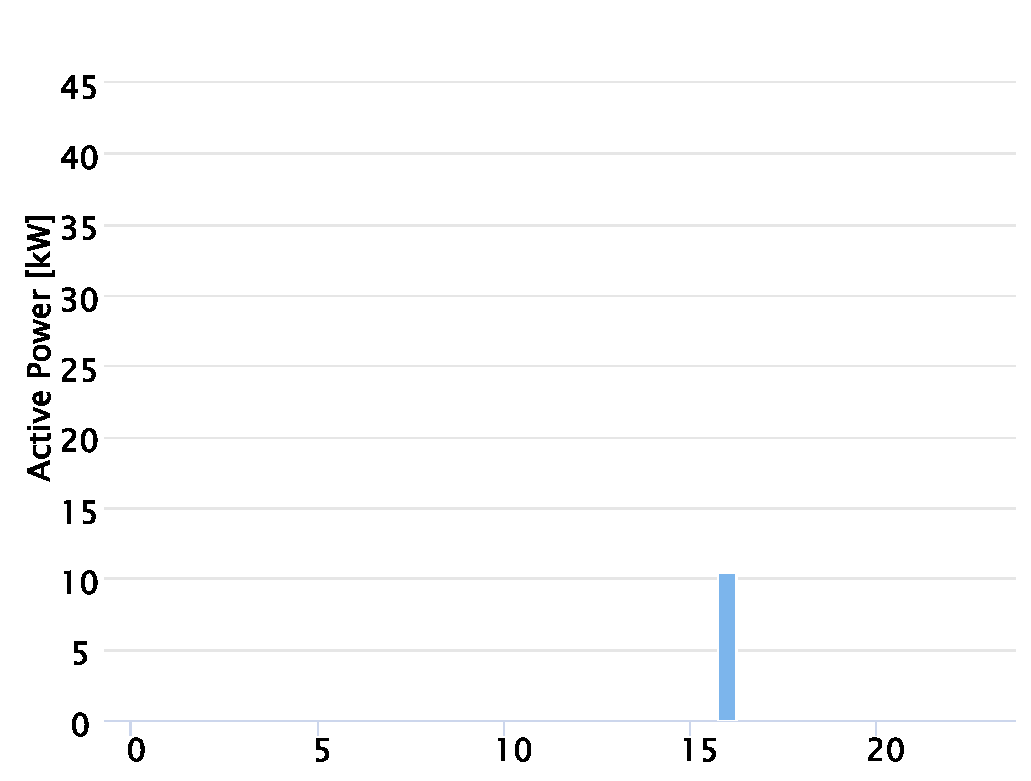
\includegraphics[width=0.45\textwidth]{Figures/5_case/pv-curtailment.pdf}
        \label{fig:case_V_pv_curt_dispatch}
    }
    \subfloat[Case VI: Contingency at 08:00 hours with \glspl{ev}.]{
        \includegraphics[width=0.45\textwidth]{Figures/6_case/pv-curtailment.pdf}
        \label{fig:case_VI_pv_curt_dispatch}
    }
    \caption{PV curtailment for each case.}
    \label{fig:pv_curtailment_dispatch}
\end{figure*}

\begin{figure*}[!htb]
    \centering
    \subfloat[Case IV: Without contingencies, including \glspl{ev}.]{
        \includegraphics[width=0.45\textwidth]{Figures/4_case/ev.pdf}
        \label{fig:case_IV_ev_dispatch}
    }
    \subfloat[Case V: Contingency at 16:00 hours with \glspl{ev}.]{
        \includegraphics[width=0.45\textwidth]{Figures/5_case/ev.pdf}
        \label{fig:case_V_ev_dispatch}
    }
    \caption{EV 2 dispatch for each case of study.}
    \label{fig:ev_dispatch}
\end{figure*}

\begin{figure*}[!htb]
    \centering
    \subfloat[EV 1]{
        \includegraphics[width=0.45\textwidth]{Figures/6_case/ev1.pdf}
        \label{fig:case_VI_ev1_dispatch}
    }
    \subfloat[EV 2]{
        \includegraphics[width=0.45\textwidth]{Figures/6_case/ev2.pdf}
        \label{fig:case_VI_ev2_dispatch}
    }
    \caption{EV dispatch for VI case of study.}
    \label{fig:ev_1_2_dispatch}
\end{figure*}


\begin{figure*}[!htb]
    \centering
    \subfloat[Case I: Without contingencies.]{
        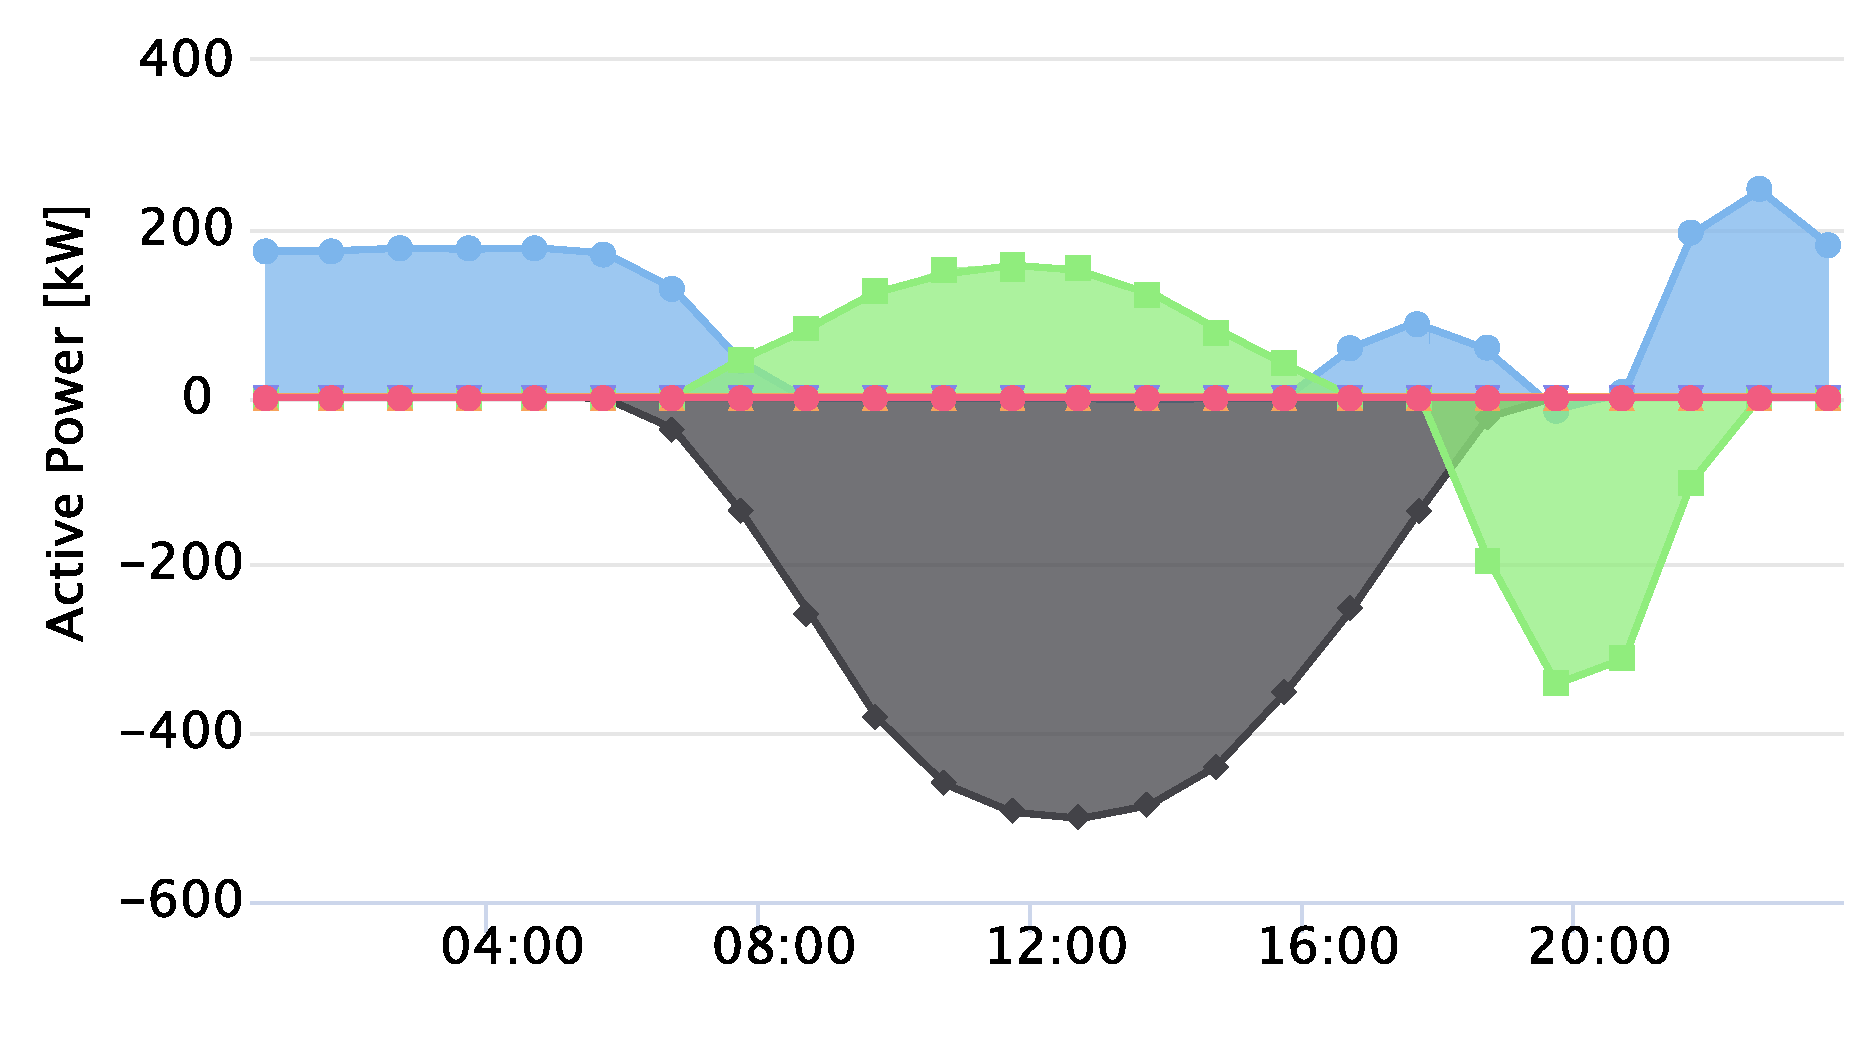
\includegraphics[width=0.45\textwidth]{Figures/1_case/microgrid-operation.pdf}
        \label{fig:case_I_operation}
    }
    \subfloat[Case II: Contingency at 16:00 hours.]{
        \includegraphics[width=0.45\textwidth]{Figures/2_case/microgrid-operation.pdf}
        \label{fig:case_II_operation}
    }
    \vfill
    \subfloat[Case III: Contingency at 08:00 hours.]{
        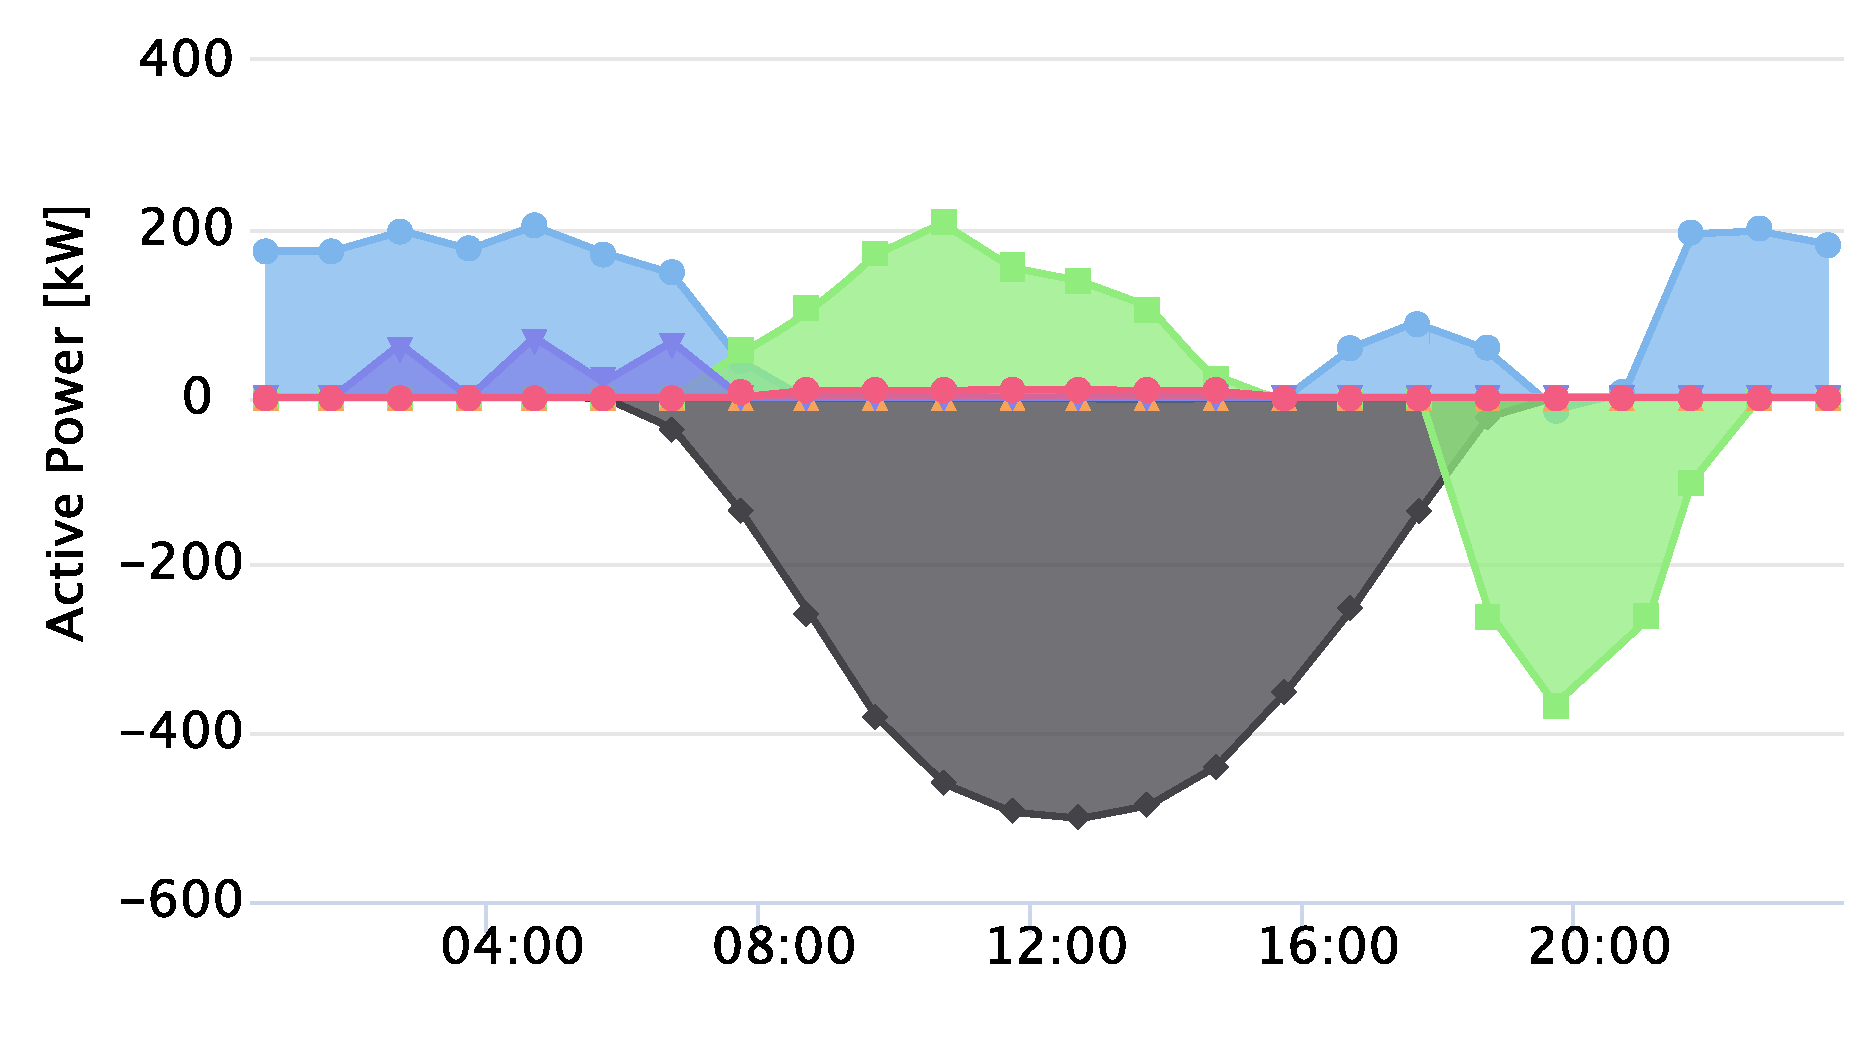
\includegraphics[width=0.45\textwidth]{Figures/3_case/microgrid-operation.pdf}
        \label{fig:case_III_operation}
    }
    \subfloat[Case IV: Without contingencies, including \glspl{ev}.]{
        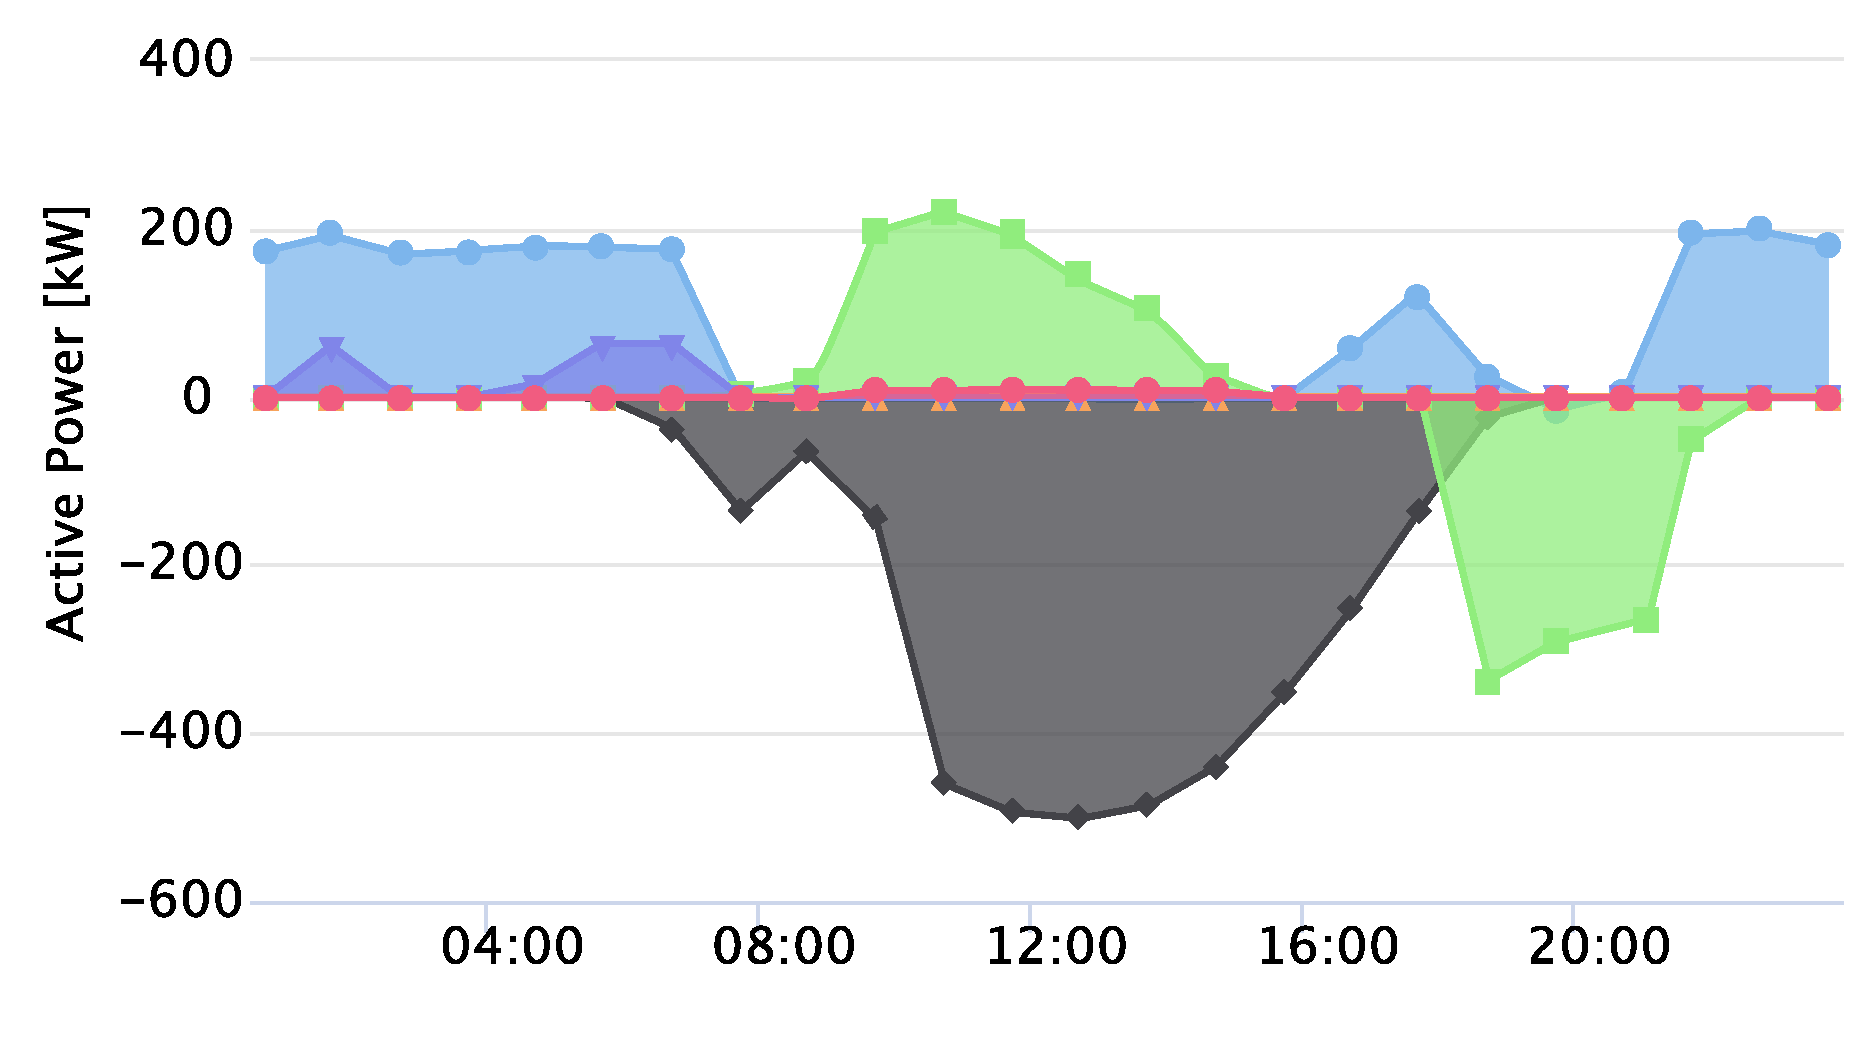
\includegraphics[width=0.45\textwidth]{Figures/4_case/microgrid-operation.pdf}
        \label{fig:case_IV_operation}
    }
    \vfill
    \subfloat[Case V: Contingency at 16:00 hours with \glspl{ev}.]{
        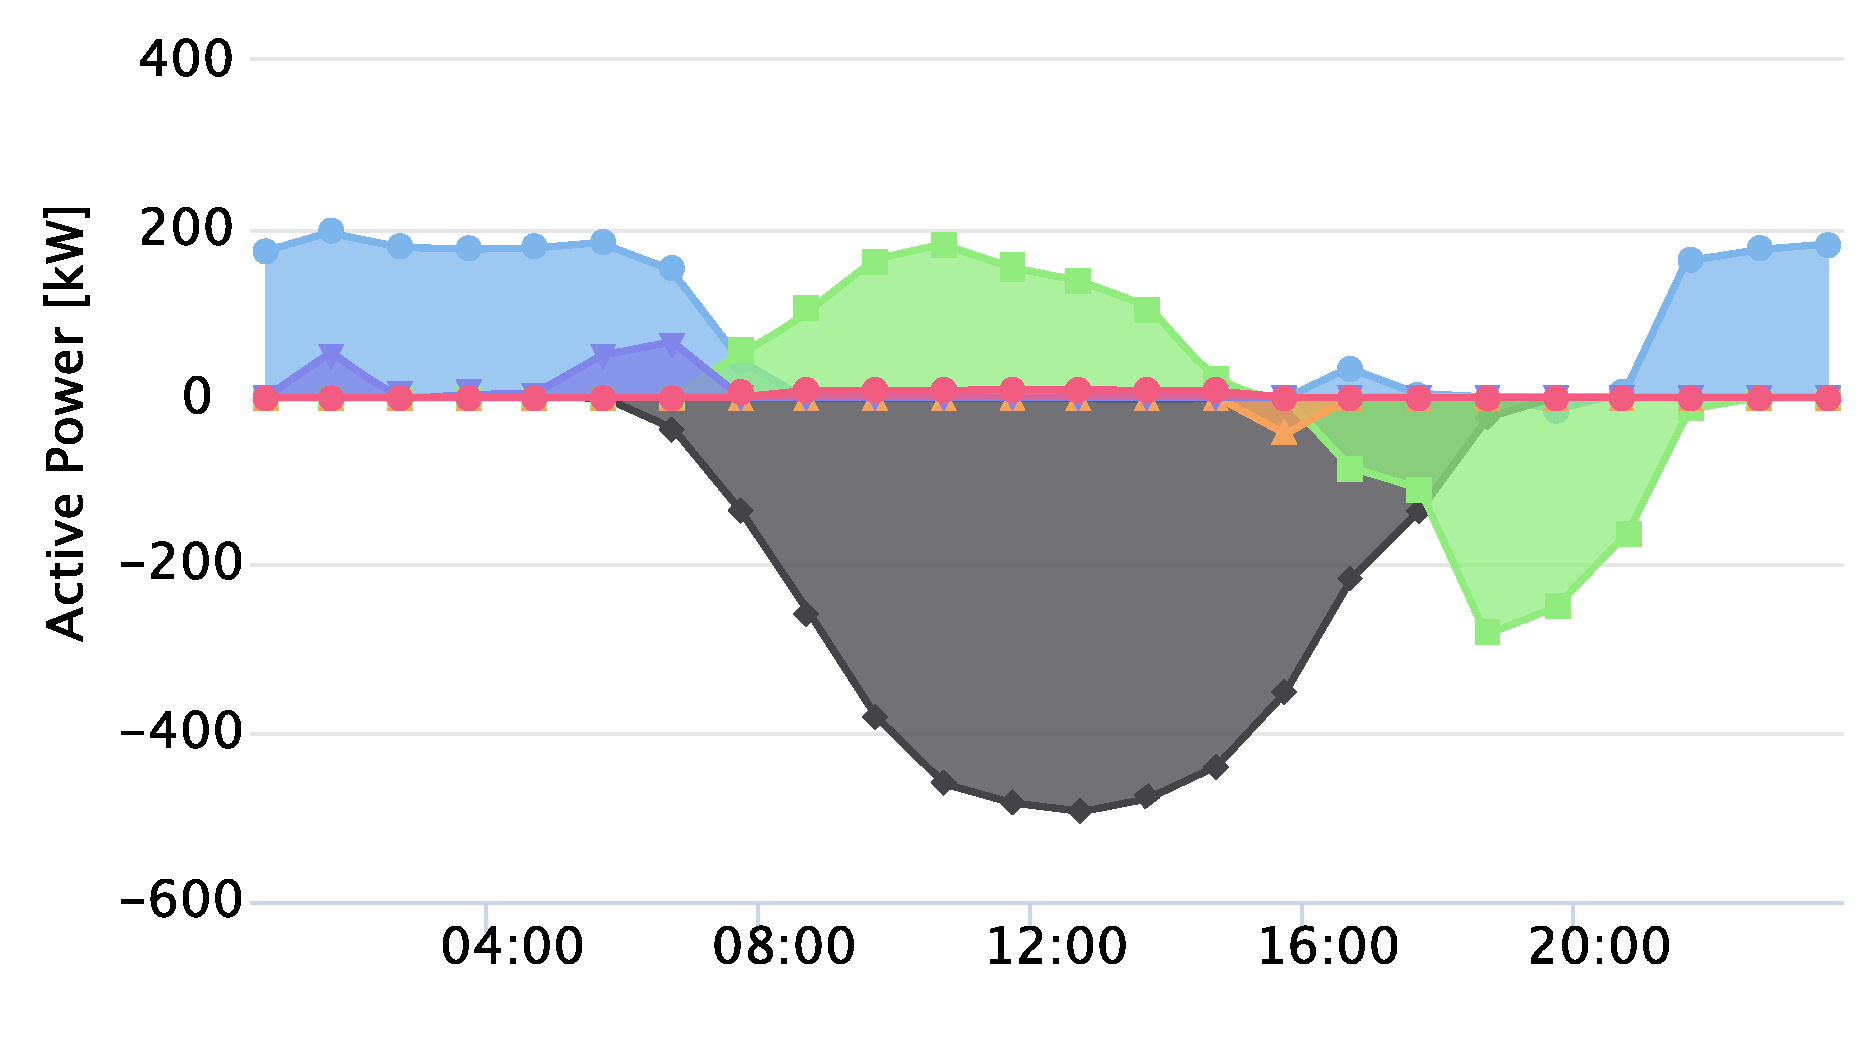
\includegraphics[width=0.45\textwidth]{Figures/5_case/microgrid-operation.pdf}
        \label{fig:case_V_operation}
    }
    \subfloat[Case VI: Contingency at 08:00 hours with \glspl{ev}.]{
        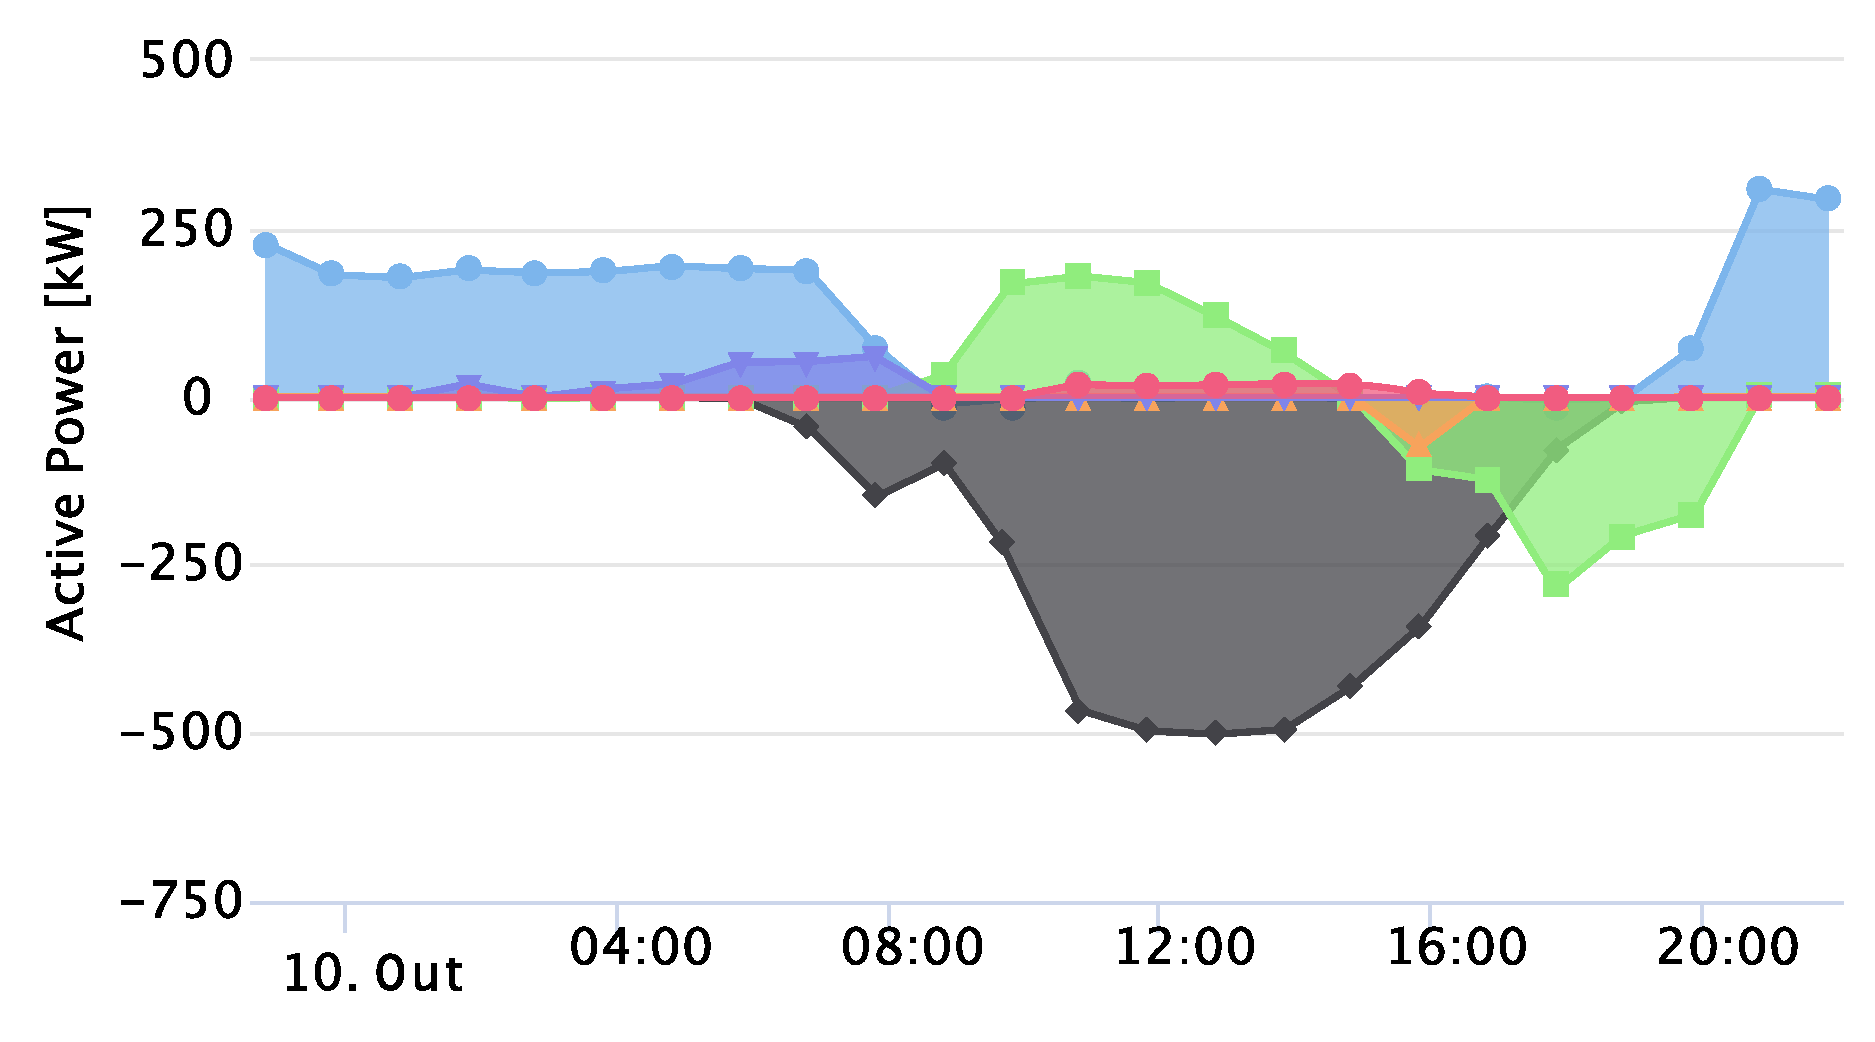
\includegraphics[width=0.45\textwidth]{Figures/6_case/microgrid-operation.pdf}
        \label{fig:case_VI_operation}
    }
    \caption{Microgrid 24 hours for each case study.}
    \label{fig:microgrid_operation}
\end{figure*}

\begin{figure*}[!htb]
    \centering
    \subfloat[Case I: Without contingencies.]{
        \includegraphics[width=0.32\textwidth]{Figures/1_case/state-of-charge.pdf}
        \label{fig:case_I_soc}
    }
    \subfloat[Case II: Contingency at 16:00 hours.]{
        \includegraphics[width=0.32\textwidth]{Figures/2_case/state-of-charge.pdf}
        \label{fig:case_II_soc}
    }
    \subfloat[Case III: Contingency at 08:00 hours.]{
        \includegraphics[width=0.32\textwidth]{Figures/3_case/state-of-charge.pdf}
        \label{fig:case_III_soc}
    }
    \vfill
    \subfloat[Case IV: Without contingencies, including \glspl{ev}.]{
        \includegraphics[width=0.32\textwidth]{Figures/4_case/state-of-charge.pdf}
        \label{fig:case_IV_soc}
    }
    \subfloat[Case V: Contingency at 16:00 hours with \glspl{ev}.]{
        \includegraphics[width=0.32\textwidth]{Figures/5_case/state-of-charge.pdf}
        \label{fig:case_V_soc}
    }
    \subfloat[Case VI: Contingency at 08:00 hours with \glspl{ev}.]{
        \includegraphics[width=0.32\textwidth]{Figures/6_case/state-of-charge.pdf}
        \label{fig:case_VI_soc}
    }
    \caption{BESS's SOC for each case of study.}
    \label{fig:soc_operation}
\end{figure*}

\begin{figure*}[!htb]
    \centering
    \subfloat[Case I: Without contingencies.]{
        \includegraphics[width=0.32\textwidth]{Figures/1_case/photovoltaic-generation.pdf}
        \label{fig:case_I_pv_generation}
    }
    \subfloat[Case II: Contingency at 16:00 hours.]{
        \includegraphics[width=0.32\textwidth]{Figures/2_case/photovoltaic-generation.pdf}
        \label{fig:case_II_pv_generation}
    }
    \subfloat[Case III: Contingency at 08:00 hours.]{
        \includegraphics[width=0.32\textwidth]{Figures/3_case/photovoltaic-generation.pdf}
        \label{fig:case_III_pv_generation}
    }
    \vfill
    \subfloat[Case IV: Without contingencies, including \glspl{ev}.]{
        \includegraphics[width=0.32\textwidth]{Figures/4_case/photovoltaic-generation.pdf}
        \label{fig:case_IV_pv_generation}
    }
    \subfloat[Case V: Contingency at 16:00 hours with \glspl{ev}.]{
        \includegraphics[width=0.32\textwidth]{Figures/5_case/photovoltaic-generation.pdf}
        \label{fig:case_V_pv_generation}
    }
    \subfloat[Case VI: Contingency at 08:00 hours with \glspl{ev}.]{
        \includegraphics[width=0.32\textwidth]{Figures/6_case/photovoltaic-generation.pdf}
        \label{fig:case_VI_pv_generation}
    }
    \caption{PV generation for each case of study.}
    \label{fig:pv_operation}
\end{figure*}

% Case VII
\begin{figure*}[!htb]
    \centering
    \subfloat[Case VII: Bess dispatch]{
        \includegraphics[width=0.45\textwidth]{Figures/7_case/bess-dispatch.pdf}
        \label{fig:case_VII_bess_dispatch}
    }
    \subfloat[Case VII: Genset dispatch]{
        \includegraphics[width=0.45\textwidth]{Figures/7_case/genset-dispatch.pdf}
        \label{fig:case_VII_genset_dispatch}
    }
    \vfill
    \subfloat[Case VII: PV curtailment]{
        \includegraphics[width=0.45\textwidth]{Figures/7_case/pv-curtailment.pdf}
        \label{fig:case_VII_pv_curtailment}
    }
    \subfloat[Case VII: EV 2 dispatch]{
        \includegraphics[width=0.45\textwidth]{Figures/7_case/ev2.pdf}
        \label{fig:case_VII_ev_2_dispatch}
    }
    \vfill
    \subfloat[Case VII: Microgrid operation 24 hours]{
        \includegraphics[width=0.45\textwidth]{Figures/7_case/microgrid-operation.pdf}
        \label{fig:case_VII_operation}
    }
    \caption{Case VII: Contingencies at 08:00 and 16:00 hours with EVs}
    \label{fig:case_VII}
\end{figure*}

\glsresetall
\section{Conclusions}\label{sec:conclusions}

A \gls{moop} has been proposed to minimizes the operational costs from the main
grid and the \gls{ens} for \glspl{ev}. The $\varepsilon$-constraint method
was applied to solve the \gls{moop} and obtain the Pareto front. The centroid
of the Pareto front was used to determine the optimal dispatch of the 
\gls{bess} and \glspl{ev} for seven case studies. 

A new tab and database table for \glspl{ev} was developed in the IoT-based 
\gls{ems}. This tab allows the user to input the \gls{ev} parameters, such as
the arrival and departure times, the maximum energy capacity, and the
\gls{ev} charging power.

All case studies were conducted using the Typhoon HIL 604 and the results were
displayed in the GUI. The \gls{bess} dispatch, genset dispatch, \gls{pv}
curtailment, and \gls{ev} charging were analyzed for each case. The microgrid's
24-hour operation, the \gls{soc} of the \gls{bess}, and the \gls{pv} generation
were also visualized.

\appendix

\section{Piecewise Linearization}\label{appndx:piecewise}

The quadratic terms $(P_{ij,f,ht,c})^2$, 
$(Q_{ij,h,t,c})^2$, $(P_{i,f,t,c}^{\text{PCC}})^2$ and  
$(Q_{i,f,t,c}^{\text{PCC}})^2$ in (\ref{I}) and 
(\ref{pcc}) are linearized using a linear piecewise approximation function as 
presented in \cite{silva2021}. To linearize the terms 
$(P_{ij,f,ht,c})^2$, $(Q_{ij,h,t,c})^2$, $(P_{i,f,t,c}^{\text{PCC}})^2$ and 
$(Q_{i,f,t,c}^{\text{PCC}})^2$, the variables 
$(P_{ij,f,ht,c}^{sqr})^2$, $(Q_{ij,h,t,c}^{sqr})^2$, 
$(P_{i,f,t,c}^{\text{PCCsqr}})^2$ and $(Q_{i,f,t,c}^{\text{PCCsqr}})^2$ is 
introduced to the model the square of the active and reactive power flow and
square of the active and reactive 
power at the PCC. Therefore, constrains related to the definition 
of variables and their limits for the piecewise linearization approximation are 
given in (\ref{pw1})-(\ref{pw6}).

\vspace{-20pt}
\begin{flalign}\label{pw1}
& f(x,\overline{x}, Y) = \sum_{y=1}^{Y} \sigma_{x,y} \cdot  \Delta_{x,y}  \ \ \ 
    \forall x& 
\end{flalign}
\vspace{-35pt}

\begin{flalign}\label{pw2}
& x = x^{+} - x^{-}  \ \ \ \forall x& 
\end{flalign}
\vspace{-40pt}

\begin{flalign}\label{pw3}
& x^{+} - x^{-} = \sum_{y=1}^{Y} \Delta_{x,y}  \ \ \ \forall x& 
\end{flalign}
\vspace{-35pt}

\begin{flalign}\label{pw4}
    & 0 \leq \Delta_{x,y} \leq \overline{x} / Y \ \ \ \forall x,y = 1, \dots, Y &
\end{flalign}
\vspace{-40pt}

\begin{flalign}\label{pw5}
    & \sigma_{x,y} = (2y - 1) \overline{x} / Y \ \ \ \forall x,y = 1, \dots, Y &
\end{flalign}
\vspace{-40pt}

\begin{flalign}\label{pw6}
    & x = x^{+} - x^{-} \geq 0 &
\end{flalign}

\subsection{Linearization of the AC power flow model}

The definition of the apparent power losses in (\ref{P_losses}) and 
(\ref{Q_losses}) is nonlinear due to multiplication of continuous variables. 
To linearize these constraints, estimated active and reactive power flows 
through lines of each phase $f$, i.e., $\Tilde{P}_{ij,h,t}P_{ij,f,t}$ and 
$\Tilde{Q}_{ij,h,t}Q_{ij,f,t}$ and, the estimated values of voltage 
magnitudes, i.e., $\Tilde{V}_{i,f,t}$ and $\Tilde{V}_{i,h,t}$ can be used. 
Thus, $P^{\text{L}}_{ij,f,t}$ and $Q^{\text{L}}_{ij,f,t}$ can be approximated 
using the linear expression given by (\ref{pw1}) and (\ref{pw2}). 

\vspace{-20pt}
\begin{multline}\label{pw_P_losses}
\hspace{-5pt} P^{\text{L}}_{ij,f,t} =  \\
\hspace{-1pt}\sum_{h \in \mathcal{F}} 
\frac{1}{\Tilde{V}_{i,f,t}\Tilde{V}_{i,h,t}}\bigg[ R'_{ij,f,h}
\Big(\Tilde{P}_{ij,h,t}P_{ij,f,t}  + \Tilde{Q}_{ij,h,t}Q_{ij,f,t}\Big) \\+  
X'_{ij,f,h} \Big( \Tilde{Q}_{ij,h,t}P_{ij,f,t} - 
\Tilde{P}_{ij,h,t}Q_{ij,f,t}\Big) 
\bigg] \ \ \ \forall ij,f,h,t
\end{multline}
\vspace{-50pt}

\begin{multline}\label{pw_Q_losses}
\hspace{-5pt}Q^{\text{L}}_{ij,f,t} = \\
\hspace{-1pt} \sum_{h \in \mathcal{F}} 
\frac{1}{\Tilde{V}_{i,f,t}\Tilde{V}_{i,h,t}}
\bigg[ R'_{ij,f,h}\Big(\Tilde{P}_{ij,h,t}Q_{ij,f,t} - 
\Tilde{Q}_{ij,h,t}P_{ij,f,t}\Big) \\+  
\hspace{-1pt} X'_{ij,f,h} \Big( \Tilde{P}_{ij,h,t}P_{ij,f,t} + 
\Tilde{Q}_{ij,h,t}Q_{ij,f,t}\Big)  \bigg] \ \ \ \forall ij,f,h,t
\end{multline}
\vspace{-15pt}

The term $V^{\text{2}}_{i,f,t,c}$ in the left-hand side of constraint 
(\ref{V_drop}) and (\ref{I}) can be linearized by introducing 
the variable $V^{\text{sqr}}_{i,f,t,c}$ to represent the square value of 
voltage magnitude. Furthermore, the terms $P_{ij,f,ht,c}^{2}$ and 
$Q_{ij,h,t,c}^{2}$ in constraint (\ref{I}) can be linearized 
introducing the variables $P^{\text{sqr}}_{ij,f,t,c}$ and 
$Q^{\text{sqr}}_{ij,f,t}$. Thus, the constraint (\ref{I}) can be 
rewritten as the linear expression in (\ref{pw_I}). Additionally, 
(\ref{V_drop}) can be rewritten as in (\ref{pc_V_droop_1}).

\vspace{-10pt}
\begin{flalign}\label{pw_I}
&\frac{\left(P^{\text{sqr}}_{ij,f,t,c} + 
Q^{\text{sqr}}_{ij,f,t,c}\right)}{V^{sqr}_{i,f,t}}  
\leq \overline{I}_{ij}^2 \ \ \ \forall ij,f,t &
\end{flalign}
\vspace{-30pt}

\begin{multline}\label{pc_V_droop_1}
\hspace{-8pt}V^{\text{sqr}}_{i,f,t,c}  - V^{\text{sqr}}_{j,f,t,c} = 
2 \sum_{h \in \mathcal{F}} \left(  R'_{ij,f,h} P_{ij,h,t}
+ X'_{ij,f,h} Q_{ij,h,t} \right)  -  \\ 
\hspace{-1pt}\frac{1}{V^{\text{2}}_{i,f,t}} 
\left[\sum_{h \in \mathcal{F}}\left(R_{ij,f,h}^{'2} + P_{ij,h,t}^{'2} \right)  
\cdot \left(P_{ij,f,h,t,c}^{2} + Q_{ij,h,t,c}^{2}\right) \right] \\
\forall ij,f,h,t
\end{multline}
\vspace{-20pt}

On the other hand, $V^{\text{2}}_{i,f,t,c}$ in the right-hand side of 
constraint (\ref{pc_V_droop_1}) is approximated based on its estimation, 
given by $\Tilde{V}_{i,f,t,c}$. As mentioned before, the terms 
$P_{ij,f,ht,c}^{2}$ and $Q_{ij,h,t,c}^{2}$ can be linearized introducing 
the variables $P^{\text{sqr}}_{ij,f,t,c}$ and $Q^{\text{sqr}}_{ij,f,t}$. 
Finally, the constraint (\ref{pc_V_droop_1}) can be rewritten as the linear 
expression in (\ref{pc_V_droop_2}).

\vspace{-20pt}
\begin{multline}\label{pc_V_droop_2}
\hspace{-8pt}V^{\text{sqr}}_{i,f,t}  - V^{\text{sqr}}_{j,f,t} = 
2 \sum_{h \in \mathcal{F}} \left(  R'_{ij,f,h} P_{ij,h,t}
+ X'_{ij,f,h} Q_{ij,h,t} \right)  -  \\ 
\hspace{-10pt}\frac{1}{\Tilde{V}_{i,f,t}} 
\left[\sum_{h \in \mathcal{F}}\left(R_{ij,f,h}^{'2} + X_{ij,h,t}^{'2} \right)  
\cdot \left(P_{ij,f,h}^{\text{sqr}} + Q_{ij,h,t}^{\text{sqr}}\right) \right] \\
\forall ij,f,h,t
\end{multline}
\vspace{-30pt}

\subsection{Linearization of the BESS model}

The nonlinear constraint (\ref{B_unimodality}) can be linearized based  on 
the binary varibles $b^{\text{Ch}}_{m,t}$ and $b^{\text{Dis}}_{m,t}$ according 
to the (\ref{pw_bess}). The binary variables are used to represents the 
operational state of the BESS in charging mode ($b^{\text{Ch}}_{m,t} = 1$) or 
discharging mode ($b^{\text{Dis}}_{m,t}$). This is enforced by constraints in 
(\ref{pw_bess_2}) and (\ref{pw_bess_3}), and constraint (\ref{pw_bess_4}) 
defines the binary nature of variables $b^{\text{Ch}}_{m,t}$ and 
$b^{\text{Dis}}_{m,t}$.    

\vspace{-15pt}
\begin{flalign}\label{pw_bess}
& b^{\text{Ch}}_{m,t} + b^{\text{Dis}}_{m,t}\leq 0 \ \ \  \forall m, t &
\end{flalign} 
\vspace{-35pt}

\begin{flalign}\label{pw_bess_2}
& 0 \leq P^{\text{B+}}_{m,t} \leq \overline{P}^{\text{B}}_{m} \ \ \  
    \forall m, t &
\end{flalign} 
\vspace{-35pt}

\begin{flalign}\label{pw_bess_3}
& 0 \leq P^{\text{B-}}_{m,t} \leq \overline{P}^{\text{B}}_{m} \ \ \   
    \forall m, t &
\end{flalign}
\vspace{-35pt}

\begin{flalign}\label{pw_bess_4}
& b^{\text{Ch}}_{m,t}, b^{\text{Dis}}_{m,t} \in  \text{0,1} \ \ \  
    \forall m, t &
\end{flalign} 
\vspace{-30pt}

\bibliographystyle{elsarticle-num}
\bibliography{5-references.bib}

\section{Work Plan and Schedule}

To accomplish the activities of this Master's degree project adequately, solid theoretical knowledge in the area of microgrids and power systems was necessary. This master's project began in the first 
semester of 2023. The courses that were taken in the first two semesters were those shown in Table \ref{tab:courses}.

\begin{table}[h]
\centering
\caption{Courses taken to complete required credits.}
\label{tab:courses}
\begin{tabular}{@{}c|l@{}}
\toprule
\multirow{2}{*}{1st} & 
\begin{tabular}[c]{@{}l@{}}IT509-A - Stochastic Processes for Engineering
    \\ (Concept B)
\end{tabular} 
    \\ \cmidrule(l){2-2} 
& \begin{tabular}[c]{@{}l@{}} IT511-A - Energy Operation of Electric Power 
    \\ Systems (Concept A)
\end{tabular}
    \\ \midrule

\multirow{3}{*}{2nd} & 
\begin{tabular}[c]{@{}l@{}}IT306-Q - Topics in Electric Power Systems III:\\
    Optimization Applied to Electric Power\\
    Distribution Systems (Concept A)
\end{tabular} 
    \\ \cmidrule(l){2-2} 
& \begin{tabular}[c]{@{}l@{}}IT306-HH - Topics in Electric Power Systems III:\\
    Energy Storage Systems (Concept A)
\end{tabular} 
    \\
\bottomrule
\end{tabular}
\end{table}

The stages of the master's works are shown below.

\begin{description}
    \item[Stage 01] Taking courses to fulfill the credit requirements.
    \item[Stage 02] Continuation of courses for required credits and 
                    introduction to the MERGE project.
    \item[Stage 03] Learning and understanding the CAMPUSGRID microgrid 
                    mathematical model using Python and Pyomo.
    \item[Stage 04] Implementation of the mathematical model with the inclusion 
                    of linearizations, contingencies and scenarios using Pyomo.
    \item[Stage 05] Gaining knowledge of the backend (Flask API and database) 
                    and frontend (Angular) technologies.
    \item[Stage 06] Preparing study cases for 24-hours simulations with software
                    Typhoon HIL604. 
    \item[Stage 07] Preparation for the qualification exam. 
    \item[Stage 08] Simulations with hardware Typhoon HIL604 in the 
                    Smart Grids Laboratory (LABREI), a rolling horizon approach
                    and PV forecasting will be included. 
    \item[Stage 09] Writing and preparation of the master thesis.
    \item[Stage 10] Defending the master's thesis.
\end{description}\par
\vspace{3 pt}

The schedule of the completed and planned stages is in Table \ref{tab:sche}. 
In addition, two papers were developed and submitted for conferences.

\begin{table}[]
\caption{Scheduled and project status}
\centering
\label{tab:sche}
\begin{tabular}{cllll}
\textbf{Stage} &
  \multicolumn{1}{c}{\textbf{\begin{tabular}[c]{@{}c@{}}1st\\ 2023\end{tabular}}} &
  \multicolumn{1}{c}{\textbf{\begin{tabular}[c]{@{}c@{}}2nd\\ 2023\end{tabular}}} &
  \multicolumn{1}{c}{\textbf{\begin{tabular}[c]{@{}c@{}}1st\\ 2024\end{tabular}}} &
  \multicolumn{1}{c}{\textbf{\begin{tabular}[c]{@{}c@{}}2nd\\ 2024\end{tabular}}} \\ 
  \hline
\multicolumn{1}{|c|}{01} &
  \multicolumn{1}{c|}{\cellcolor[HTML]{bdc6d1}} &
  \multicolumn{1}{c|}{} &
  \multicolumn{1}{c|}{} &
  \multicolumn{1}{c|}{} \\ \hline
\multicolumn{1}{|c|}{02} &
  \multicolumn{1}{c|}{} &
  \multicolumn{1}{c|}{\cellcolor[HTML]{bdc6d1}} &
  \multicolumn{1}{c|}{} &
  \multicolumn{1}{c|}{} \\ \hline
\multicolumn{1}{|c|}{03} &
  \multicolumn{1}{l|}{} &
  \multicolumn{1}{c|}{\cellcolor[HTML]{bdc6d1}} &
  \multicolumn{1}{c|}{} &
  \multicolumn{1}{l|}{} \\ \hline
\multicolumn{1}{|c|}{04} &
  \multicolumn{1}{l|}{} &
  \multicolumn{1}{l|}{\cellcolor[HTML]{bdc6d1}} &
  \multicolumn{1}{c|}{} &
  \multicolumn{1}{l|}{} \\ \hline
\multicolumn{1}{|c|}{05} &
  \multicolumn{1}{l|}{} &
  \multicolumn{1}{l|}{} &
  \multicolumn{1}{c|}{\cellcolor[HTML]{bdc6d1}} &
  \multicolumn{1}{l|}{} \\ \hline
\multicolumn{1}{|c|}{06} &
  \multicolumn{1}{l|}{} &
  \multicolumn{1}{l|}{} &
  \multicolumn{1}{c|}{\cellcolor[HTML]{bdc6d1}} &
  \multicolumn{1}{l|}{} \\ \hline
\multicolumn{1}{|c|}{07} &
  \multicolumn{1}{l|}{} &
  \multicolumn{1}{l|}{} &
  \multicolumn{1}{l|}{\cellcolor[HTML]{bdc6d1}} &
  \multicolumn{1}{c|}{} \\ 
  \hline
\multicolumn{1}{|c|}{08} &
  \multicolumn{1}{l|}{} &
  \multicolumn{1}{l|}{} &
  \multicolumn{1}{l|}{} &
  \multicolumn{1}{c|}{\cellcolor[HTML]{ffb703}}\\ 
  \hline
\multicolumn{1}{|c|}{09} &
  \multicolumn{1}{l|}{} &
  \multicolumn{1}{l|}{} &
  \multicolumn{1}{l|}{} &
  \multicolumn{1}{l|}{\cellcolor[HTML]{ffb703}} \\ 
  \hline
\multicolumn{1}{|c|}{10} &
  \multicolumn{1}{l|}{} &
  \multicolumn{1}{l|}{} &
  \multicolumn{1}{l|}{} &
  \multicolumn{1}{l|}{\cellcolor[HTML]{ffb703}} \\ 
  \hline
&&&&\\
 &
  \multicolumn{2}{c}{\cellcolor[HTML]{bdc6d1}Done} &
  \multicolumn{2}{c}{\cellcolor[HTML]{ffb703}To do}
\end{tabular}
\end{table}

\begin{enumerate}
    \item \textbf{Gerenciamento de Energia em Tempo Real da 
    Microrrede LABREI}, Published in "Congresso Brasileiro de Energia 
    Solar", Natal RN, 2024.\\
    Authors: Jéssica Alice A. Silva, Derian C. Tairo, Juan Camilo López,
    Guilherme S. Chagas, Marcos J. Rider, Luiz C. P. da Silva. 
    \item \textbf{Stochastic Optimization of Energy Resources in Smart Homes},
    Accepted to the IEEE ANDESCON, Cusco - Perú, 2024.\\
    Authors: Jéssica Alice A. Silva, Derian C. Tairo,
    Guilherme S. Chagas, Marcos J. Rider.

\end{enumerate}

\end{document}